\documentclass[11pt]{article}
\usepackage[letterpaper,margin=1in]{geometry}
\usepackage[T1]{fontenc}
\usepackage{mathptmx}
\usepackage[scaled=0.9]{helvet}
\usepackage{courier}
\usepackage{placeins}
\renewcommand{\topfraction}{0.9}\renewcommand{\bottomfraction}{0.8}\renewcommand{\textfraction}{0.07}\renewcommand{\floatpagefraction}{0.75}\setcounter{topnumber}{3}\setcounter{totalnumber}{5}
\usepackage{ragged2e}
\usepackage{microtype}
\usepackage{amsmath}
\usepackage{graphicx}
\usepackage{booktabs}
\usepackage{threeparttable}
\usepackage{array}
\usepackage{tabularx}
\usepackage{multirow}
\usepackage{makecell}
\usepackage[table]{xcolor}
\usepackage{enumitem}
\usepackage[font=small,labelfont=bf,labelsep=period,justification=justified,singlelinecheck=false]{caption}
\usepackage[numbers,sort&compress]{natbib}
\usepackage{authblk}
\usepackage{titlesec}
\usepackage{fancyhdr}
\usepackage[colorlinks=true,linkcolor=blue!50!black,citecolor=blue!50!black,urlcolor=blue!50!black]{hyperref}

\definecolor{rowgray}{HTML}{F3F2EF}
\definecolor{accent}{HTML}{2A78D6}
\linespread{1.12}
\setlength{\parskip}{3pt}
\setlist{itemsep=2pt,topsep=3pt}
\titleformat{\section}{\normalfont\large\bfseries\sffamily}{\thesection}{0.6em}{}
\titleformat{\subsection}{\normalfont\normalsize\bfseries\sffamily}{\thesubsection}{0.6em}{}
\titlespacing*{\section}{0pt}{14pt}{5pt}
\titlespacing*{\subsection}{0pt}{9pt}{3pt}
\renewcommand{\arraystretch}{1.15}
\setlength{\tabcolsep}{5pt}
\newcommand{\RR}{R\textsuperscript{2}}
\newcommand{\mgdl}{mg/dL}
\pagestyle{fancy}\fancyhf{}
\fancyhead[L]{\small\sffamily Reassessing PPG-based glucose estimation}
\fancyhead[R]{\small\sffamily Manuscript draft, 8 November 2026}
\fancyfoot[C]{\small\thepage}
\renewcommand{\headrulewidth}{0.4pt}

\title{\sffamily\bfseries Reassessing PPG-based blood glucose estimation: patient-independent validation, optical modelling and embedded implementation}
\author[1]{Mohammad Ghamari}
\author[1]{Milan Chhetri}
\author[1]{Souvik Kundu}
\author[2]{Khalil Alipour}
\author[2]{Bahram Tarvirdizadeh}
\affil[1]{Department of Electrical Engineering, California Polytechnic State University, San Luis Obispo, CA, USA}
\affil[2]{Advanced Service Robots (ASR) Laboratory, Department of Mechatronics Engineering, School of Intelligent Systems Engineering, College of Interdisciplinary Science and Technology, University of Tehran, Tehran, Iran}
\date{}

\begin{document}
\maketitle
\thispagestyle{fancy}

\begin{abstract}
\noindent Deep networks on photoplethysmography (PPG) have been reported to estimate blood glucose with errors near 20~\mgdl{}, including in our own previous work. We extended that work to patient-wise evaluation on 7,224 intra-operative laboratory glucose readings from 2,991 VitalDB patients, and asked how much glucose information PPG carries for unseen patients, where it comes from, and what limits it. ResNet34-1D reached \RR{} 0.23 with segment-level splits but 0.04 on unseen patients, no better than age, sex and body-mass index; far beyond seed-to-seed variation. Two pretrained PPG foundation models, frozen or fine-tuned, did no better. Clinical context plus PPG features reached RMSE 31.8~\mgdl{}, with PPG contributing 1.1~\mgdl{} (95\% CI 0.7 to 1.5). This information was shared with electrocardiogram, arterial pressure and monitor signals. With one reference glucose value per patient, adding the change in PPG features lowered RMSE from 33.0 to 31.3~\mgdl{} on the same readings, but hypoglycaemia sensitivity was at most 3.4\%. On the external MUST dataset no model beat a constant prediction. A Monte Carlo model of three-layer skin indicated, under its assumptions (including no glucose absorption below 1000~nm in the main model), a model-derived glucose-equivalent error of at least 71~\mgdl{} for any single wavelength. A wearable-input model ran on an ESP32-S3 in 0.3~s per minute of PPG, with outputs identical to Python on all 30 test recordings. In the datasets and models evaluated, clinical PPG at oximeter wavelengths carried little person-independent glucose information, consistent with predominantly haemodynamic correlates rather than direct glucose sensing.
\end{abstract}

\noindent\textbf{Keywords:} photoplethysmography; non-invasive glucose monitoring; subject-wise validation; generalisation; Monte Carlo simulation; embedded machine learning

% =====================================================================
\section{Introduction}
Non-invasive glucose monitoring would remove the finger-prick and sensor-insertion burden of diabetes care. Photoplethysmography (PPG) is attractive because almost every wearable already measures it~\citep{allen2007,castaneda2018}. Several studies report clinically acceptable glucose estimates from PPG~\citep{montemoreno2011,chu2021,gupta2021,prabha2022}, including with deep networks alone, most recently a ResNet34-1D trained on 1-s beat segments from the VitalDB surgical database~\citep{zeynali2025,lee2022vitaldb}.

The physical case for this is weak. Glucose absorbs mainly above 1000~nm~\citep{amerov2004}, whereas clinical pulse oximeters measure at about 660 and 940~nm~\citep{jubran2015}, where the nearest glucose bands overlap with temperature-sensitive water bands~\citep{golic2003}. Glucose also lowers tissue scattering slightly by reducing the refractive-index mismatch between cells and interstitial fluid~\citep{kohl1994,larin2003}, but in our Monte Carlo model of the sensor geometry a 1~mmol/L (18~\mgdl{}) change alters the modelled near-infrared reflectance by only about 0.04 to 0.18\% (Section~\ref{sec:simres}), a calculated rather than a measured response. Any reported accuracy therefore needs an evaluation that rules out shortcuts.

A central question is how the data are split. When segments from one person, often from one glucose reading, appear in both the training and the test set, a model can partly recognise the person's waveform and recall their glucose. Such record-wise splitting estimates performance on people already seen in training, whereas subject-wise splitting estimates performance on new people; the two can differ widely in clinical machine learning~\citep{saeb2017,kapoor2023}. Ramesh et al.~\citep{ramesh2026} recently reimplemented five published PPG-glucose methods, including ours, and showed that all of them reach near-zero or negative \RR{} under participant-aware splits, and that Clarke error-grid zones A+B do not distinguish the two settings. Their work, published at ISWC 2026, establishes this effect across methods, so it is not the main contribution of this paper. We ask a follow-on question: \emph{for patients not seen in training, how much glucose information does clinical PPG carry, where does it come from, and is the limit physiological, optical or computational?} As authors of one of these studies, we answer it starting from our own released code, with four kinds of evidence that a re-implementation cannot provide: the original pipeline evaluated under both protocols, controlled comparisons against every other signal recorded at the bedside with and without calibration, an optical model of what a PPG can sense, and a bit-exact embedded implementation.

\noindent\textbf{Related work.} Table~\ref{tab:related} summarises representative PPG-glucose studies. Most report Clarke zone A+B close to 100\% and validate with random splits of recordings or segments, so the same people appear in training and testing; studies that hold out people or days report far weaker accuracy, and person-specific models are validated on very few participants. Embedded deployment is rare; our previous study~\citep{zeynali2025} ran a ResNet34 on an STM32H7 microcontroller.

\begin{table}[!htbp]
\centering\footnotesize\setlength{\tabcolsep}{3.5pt}
\begin{threeparttable}
\caption{Representative PPG-based glucose studies and the validation they used.}
\label{tab:related}
\begin{tabularx}{\linewidth}{@{}>{\RaggedRight}p{0.15\linewidth}>{\RaggedRight}p{0.10\linewidth}>{\RaggedRight}p{0.15\linewidth}>{\RaggedRight}p{0.10\linewidth}>{\RaggedRight}p{0.17\linewidth}>{\RaggedRight}X@{}}
\toprule
Study & People & Signal & Model & Validation & Reported accuracy \\
\midrule
Monte-Moreno, 2011~\citep{montemoreno2011} & 410 & Fingertip PPG + physiological data & Random forest & Cross-validation & Clarke A 87.7\%, B 10.3\% \\
Chu et al., 2021~\citep{chu2021} & 2,538 & Fingertip PPG, 2 $\times$ 1~min & CNN + 17 features & Random 9:1 split, unit not stated & All 2,538 subjects: A 60.6\%; about 10 points higher with quarterly HbA1c; best subgroup with HbA1c: A 94.3\%, RMSE 12.4 \\
Gupta et al., 2021~\citep{gupta2021} & 26 & PPG & XGBoost & Leave-one-person-out, random and personalised\tnote{a} & A 96.2\%, A+B 100\%\tnote{a} \\
Prabha et al., 2022~\citep{prabha2022} & 217 & Wristband PPG + physiological data & XGBoost & Leave-subjects-out\tnote{a} & \RR{} 0.99, A 99.0\%\tnote{a} \\
Hammour \& Mandic, 2023~\citep{hammour2023} & 4 & In-ear PPG, 880~nm & Per-person regression trees & Within person; last 2 days held out & A about 80\%, A+B 100\%, RMSE 17.5--42.8 \\
Zeynali et al., 2025~\citep{zeynali2025} & 6,388 + 23 & Finger PPG (VitalDB; MUST) & ResNet34-1D & Random segment split; MUST external & VitalDB: RMSE 27.5, \RR{} 0.40, A 72.6\%; MUST: RMSE 19.7, A+B 100\%. STM32H7, 6.4~s \\
Ramesh et al., 2026~\citep{ramesh2026} & VitalDB, MUST & Reimplemented 5 methods & As published & Random vs participant-aware vs leave-subjects-out & \RR{} up to 0.60 random; $\leq$0.05 for all five under person-aware splits \\
\rowcolor{rowgray} This work & 2,991 + 23 & Finger PPG, ECG, arterial pressure, monitor, drugs; optical simulation & CNNs, gradient boosting & Person-level 5-fold; MUST external & \RR{} 0.04 (ResNet) to 0.23 (all signals); calibrated RMSE 30.8, \RR{} 0.325; ESP32-S3, 0.3~s, bit-exact \\
\bottomrule
\end{tabularx}
\begin{tablenotes}\footnotesize
\item RMSE in \mgdl{}; A, B: Clarke error-grid zones. \item[a] Values as tabulated by Ramesh et al.~\citep{ramesh2026}.
\end{tablenotes}
\end{threeparttable}
\end{table}

\noindent\textbf{Contributions.} Under this question the paper makes four linked contributions.
\begin{enumerate}[leftmargin=*]
\item \emph{Patient-wise re-evaluation.} The pipeline of our previous study~\citep{zeynali2025} evaluated on patients not seen in training, with a factorial comparison that changes only the data split, holding preprocessing and scoring fixed, on 7,224 readings of 2,991 patients, with participant flow, constant, demographic and clinical baselines, causal (pre-measurement) inputs, repeated training seeds, two pretrained PPG foundation models, and patient-level bootstrap confidence intervals.
\item \emph{Where the remaining information comes from.} Incremental and leave-one-group-out analyses of every signal recorded at the time of a glucose draw, with and without one calibration value and with a no-PPG control, plus Bland--Altman, subgroup and hypo-/hyperglycaemia detection analyses.
\item \emph{Why PPG at oximeter wavelengths is limited, under explicit optical assumptions.} A Monte Carlo analysis of three-layer skin (660 to 1700~nm) that expresses physiological confounders as glucose-equivalent errors and explains, through the rank of the sensitivity matrix, how many wavelengths are needed to separate glucose in the modelled tissue.
\item \emph{Whether computation is a barrier.} A wearable-input model in plain C on an ESP32-S3, bit-for-bit identical to Python, with hardware-in-the-loop latency and memory measurements.
\end{enumerate}
Tables and figures numbered with the prefix S are in the Supplementary Material. Figure~\ref{fig:overview} summarises the study.

\begin{figure}[!htbp]
\centering
\includegraphics[width=\linewidth]{figs/fig1_overview.pdf}
\caption{Study overview. Row 1 (evaluation): VitalDB and MUST are re-analysed with the original pipeline~\citep{zeynali2025}, changing mainly the split (schematic: 20 segments from 5 patients; a random split puts segments of the same patients in training and testing, a person-level split does not); split by person, ResNet34-1D explains no more glucose variance than age, sex and BMI. Row 2 (physics): a Monte Carlo model of three-layer skin with one source and five detectors gives the glucose-equivalent error of everyday confounders at each wavelength and detector distance (heat map, darker = larger error); in the modelled tissue one wavelength cannot isolate glucose, which becomes identifiable only with four or more (a model-dependent result). Row 3 (embedded): the wearable-input model runs on an ESP32-S3 in 0.3~s per minute of signal, with outputs identical to Python on all tested recordings. All inset charts use the results of Sections~\ref{sec:leak}, \ref{sec:simres} and \ref{sec:esp}; the PPG trace is real data from VitalDB case 1.}
\label{fig:overview}
\end{figure}

% =====================================================================
\section{Data and evaluation}
\label{sec:methods}
\subsection{Datasets}
\textbf{VitalDB.} VitalDB~\citep{lee2022vitaldb} is an open database of vital signs recorded during surgery at Seoul National University Hospital. Intra-operative laboratory glucose values (\texttt{gluc}, 20 to 600~\mgdl{}) were paired with the finger PPG waveform (\texttt{SNUADC/PLETH}, 500~Hz). A window of $\pm$8~min around each draw was decimated to 100~Hz with an anti-aliasing filter. Readings without a complete window or with fewer than 10 accepted beats were excluded. The final cohort has 7,224 readings from 3,078 surgical cases of 2,991 patients; mean glucose is 120.7~\mgdl{} (SD 35.7). Figure~\ref{fig:flow} gives the participant flow. VitalDB contains 6,388 surgical cases of 6,090 patients; the ``6,388 subjects'' of the original study~\citep{zeynali2025} is the number of cases in the database, not of patients with usable glucose and PPG data.

\begin{figure}[!htbp]
\centering
\includegraphics[width=\linewidth]{figs/fig_flow.pdf}
\caption{Participant flow. (a)~VitalDB development cohort: a reading is one laboratory glucose value with its PPG window, and a patient may contribute several readings and several surgical cases. All readings of a patient are assigned to the same cross-validation fold. (b)~MUST, used only as an external test set: all 67 recordings and the 48 recordings with at least 3 accepted beats, on which every model can be scored (Section~\ref{sec:must}).}
\label{fig:flow}
\end{figure}

\textbf{MUST.} The MUST dataset~\citep{must2023} contains 67 fingertip PPG recordings of 23 people (about 10~s each, sampled at about 2.2~kHz: 2,175~Hz as stated in~\citep{zeynali2025}, 2,190~Hz from the file lengths) with an invasive glucose value per recording (88 to 183~\mgdl{}). It was used only as an external test set. Signals were matched to labels by file name: of the 68 signal files, 67 have a glucose label.

\subsection{Preprocessing}
The original preprocessing~\citep{zeynali2025} was reproduced with one adaptation, the minimum peak spacing described below: third-order Butterworth band-pass filter, 0.5 to 8~Hz, applied forwards and backwards (zero phase); robust z-score; peak detection with a minimum spacing of 0.4~s and a prominence of 0.8; 1-s windows centred on a peak and containing exactly one peak; a template equal to the mean window; rejection of windows with cosine similarity below 0.85; and scaling of each kept beat to $[-1,1]$. The original minimum spacing of 0.8~s prevents the detection of successive peaks less than 0.8~s apart (heart rates above 75~bpm) and was therefore relaxed to 0.4~s; the pipeline evaluated here is therefore an adapted version of the original, and the same adapted pipeline is used under both splits. Figure~S1a,b shows the result on a VitalDB recording.

\subsection{Data splits}
Table~\ref{tab:splits} lists the three evaluation protocols. All person-level results use the same five folds, assigned by VitalDB \texttt{subjectid} so that patients with several operations stay in one fold; the validation set for early stopping is also split by person.

\begin{table}[!htbp]
\centering\small
\caption{Evaluation protocols.}
\label{tab:splits}
\begin{tabularx}{\linewidth}{@{}l>{\RaggedRight}X>{\RaggedRight}X@{}}
\toprule
Protocol & Unit that is split & Purpose \\
\midrule
Segment-level (original) & 1-s beats or 10-s segments, random 70/15/15 & Protocol of the original study \\
Reading-random & Glucose readings, 5-fold & Readings of one person in training and test \\
Person-level & Patients (\texttt{subjectid}), 5-fold & Performance on people not seen in training \\
\bottomrule
\end{tabularx}
\end{table}

\subsection{Models}
Figure~\ref{fig:arch} shows the four model families layer by layer, and Table~\ref{tab:models} gives their configuration and training settings.


\begin{figure}[!htbp]
\centering
\includegraphics[width=0.84\linewidth]{figs/fig_arch.pdf}
\caption{Model architectures. (a) ResNet34-1D as in the original study~\citep{zeynali2025}: a stem convolution, four residual stages with 3, 4, 6 and 3 basic blocks, global average pooling (GAP) and a dense head; it predicts glucose for each 1-s beat and a reading's estimate is the median over its beats. Labels give channels $\times$ samples after each block; italic numbers are parameter counts (\textdagger{} including the stem; the head has 164~k). (b) The residual basic block. The first convolution has stride $s=2$ in the first block of stages 2 to 4 (halving the length), and the shortcut then uses a $1\times1$ convolution with batch normalisation; elsewhere $s=1$ and the shortcut is the identity. (c) TinyCNN: four stride-2 convolutions (kernel sizes 7, 5, 5, 3; `k7/2' denotes kernel 7, stride 2), each followed by batch normalisation and ReLU; on the ESP32-S3 it takes 15~ms per beat. (d) Multi-beat CNN: the TinyCNN encoder is applied to every beat of a reading, and the mean and standard deviation of the beat embeddings feed the regression head. (e) Device model: the firmware computes 15 features from a 60-s window and sums the outputs of 300 regression trees; the calibrated variant also receives the calibration value, the minutes since it and the feature changes (timing in Section~\ref{sec:esp}). Dropout and training settings are in Table~\ref{tab:models}.}
\label{fig:arch}
\end{figure}

\begin{table}[!htbp]
\centering\footnotesize\setlength{\tabcolsep}{3.5pt}
\caption{Model configurations and training settings.}
\label{tab:models}
\begin{tabularx}{\linewidth}{@{}>{\RaggedRight}p{0.17\linewidth}>{\RaggedRight}X>{\RaggedRight}p{0.10\linewidth}>{\RaggedRight}p{0.30\linewidth}@{}}
\toprule
Model & Architecture & Parameters & Training \\
\midrule
ResNet34-1D~\citep{zeynali2025,he2016} & Conv 64 (k3), four residual stages of 3, 4, 6 and 3 basic blocks (64, 128, 256, 512 channels), global average pooling, MLP 256--128--1 with dropout 0.5; optional age, sex, BMI concatenated before the MLP & 7.38 M & AdamW (learning rate $10^{-3}$, weight decay $10^{-4}$), batch 512, up to 40 epochs, learning rate halved after 3 epochs without improvement, early stopping after 6; 32 beats per reading per epoch; MSE on standardised glucose \\
TinyCNN & Four stride-2 convolutions (16, 24, 32, 48 channels; kernels 7, 5, 5, 3) with batch normalisation and ReLU, global average pooling, MLP 32--1 with dropout 0.2 & 12.3 k & As ResNet34-1D \\
Multi-beat CNN & TinyCNN encoder shared across up to 120 beats, mean and SD pooling over beats, MLP 32--1 with dropout 0.2; optional age, sex, BMI & 13.9 k & AdamW (learning rate $10^{-3}$, weight decay $10^{-4}$), up to 40 epochs, best validation epoch kept \\
Gradient boosting, PPG baselines & Histogram gradient boosting, up to 400 trees, learning rate 0.05, $\leq$31 leaves, $\geq$40 samples per leaf, L2 1.0, internal early stopping & -- & 17 PPG features $\pm$ age, sex, BMI \\
Gradient boosting, multi-signal & 400 trees, learning rate 0.04, $\leq$15 leaves, $\geq$40 samples per leaf, L2 1.0 & -- & Feature groups of Section~\ref{sec:signals} \\
Device model & 300 trees, learning rate 0.05, $\leq$15 leaves, $\geq$40 samples per leaf, L2 1.0 & 8,700 nodes & 15 PPG features + profile (calibrated: + fingerstick terms) \\
\bottomrule
\end{tabularx}
\end{table}

\textbf{Deep networks.} ResNet34-1D (7.38~M parameters, the published architecture~\citep{zeynali2025,he2016}); the same network with age, sex and BMI fused before the regression head; TinyCNN (12.3~k parameters, four strided convolutions) sized for a microcontroller; and a multi-beat (deep-set~\citep{zaheer2017}) CNN that pools the embeddings of up to 120 beats per reading. Networks were trained in PyTorch~\citep{paszke2019} with AdamW~\citep{loshchilov2019}, mean-squared error on standardised glucose, early stopping on the person-level validation set, and 32 randomly drawn beats per reading per epoch.

\textbf{Pretrained PPG foundation models.} To test whether a larger, pretrained encoder finds information that these task-specific networks miss, we evaluated two open PPG foundation models: PaPaGei-S~\citep{pillai2025}, pretrained on 57,641~h of PPG from VitalDB, MIMIC-III and MESA (5.0~M encoder parameters; 10-s inputs at 125~Hz), and Pulse-PPG~\citep{saha2025}, pretrained on wrist PPG from a 100-day field study of 120 people (28.5~M parameters; 50~Hz). VitalDB was part of the pretraining data of PaPaGei-S (without glucose labels), which can only favour that model here. The encoders were re-implemented and the released weights loaded by parameter name, with every parameter matched. Each model received the same 10-s segments as the 10-s ResNet34-1D, z-scored and resampled to its input rate, and the 512-dimensional embeddings were averaged over the segments of a reading. The embeddings were used in three ways: frozen, with ridge regression (penalty chosen by inner cross-validation grouped by patient), with and without age, sex and BMI; frozen and reduced to 32 principal components fitted within each training fold, in the clinical-context and calibrated gradient-boosting models in place of or in addition to the hand-crafted PPG features (for the calibrated models together with their change since the calibration window); and fine-tuned end to end (PaPaGei-S with a linear head, AdamW with learning rates $10^{-4}$ for the encoder and $10^{-3}$ for the head, Huber loss, six segments per reading per epoch, up to eight epochs with early stopping on 10\% of the training patients, and the median over segments as a reading's estimate), with and without age, sex and BMI. All used the same person-level folds.

\textbf{Baselines.} The training-set mean; ridge regression on age, sex and BMI; carrying the pre-operative glucose forward; and gradient boosting~\citep{friedman2001,pedregosa2011} on 17 hand-crafted PPG features (heart rate, variability, rise time, pulse width, second-derivative ratios~\citep{elgendi2012} and signal quality~\citep{elgendi2016}), with and without demographics.

\textbf{Clinical context.} Age, sex, BMI, pre-operative diabetes, ASA physical status and emergency status from the VitalDB case table, and minutes since the start of anaesthesia. Time since anaesthesia captures surgical stress hyperglycaemia~\citep{duggan2017} and is specific to the operating room.

\textbf{Multi-signal features.} For the same readings, each case file was downloaded once and features were computed without storing waveforms. From $\pm$8~min of ECG lead II, radial arterial pressure and PPG at 100~Hz: heart rate, SDNN and RMSSD~\citep{taskforce1996} (R-peaks with a T-wave rejection rule), systolic, diastolic and mean pressure, pulse pressure, maximum $dP/dt$, and pulse arrival times~\citep{mukkamala2015} from the R-peak to the arterial and PPG peaks. From the monitor numerics in the 10~min before each draw: temperature, SpO\textsubscript{2}, end-tidal CO\textsubscript{2}, bispectral index (BIS), heart rate and mean pressure, plus their change over the preceding 30~min. From the infusion pumps in the same 10~min: propofol, remifentanil and vasopressor rates. Sensor artefacts (temperature below 30~\textdegree C, BIS of 0) were set to missing, and features recorded in fewer than 2\% of readings were dropped. Groups of features were added one at a time to a gradient-boosting model (400 trees, 15 leaves, learning rate 0.04). Because this incremental analysis depends on the order in which groups are added, each group was also left out of the full model in turn (leave-one-group-out), which measures the information unique to that group.

\textbf{Causal inputs.} The main analysis uses a window centred on each draw ($\pm$8~min), which suits a retrospective association study but not a real-time estimator. The PPG features were therefore recomputed from signal recorded only before the recorded sample time (the last 8, 2 and 1~min) and the clinical-context and calibrated models were re-evaluated with them. Monitor and drug features already use only the 10~min before each draw; the ECG and arterial features and the deep networks use the centred window. The device model (Section~\ref{sec:device}) uses the minute immediately before the recorded time. The recorded time of a laboratory value may differ from the actual blood draw; these windows are therefore causal with respect to the recorded time, and only approximately with respect to sampling.

\textbf{Calibrated models.} For patients with two or more readings, the first laboratory value serves as a single reference value (single-reference calibration) and only later readings are scored. This is a retrospective surrogate for the intended practical use, a fingerstick calibration, and was not tested prospectively (4,233 readings of 2,073 patients). Of these, 4,034 come from the same operation as the calibration, a median of 120~min later (interquartile range 81 to 188~min); 199 come from a later operation of the same patient, for which elapsed time is unknown and an indicator marks the case. RMSE of the best calibrated model is 30.1~\mgdl{} within the same operation and 42.6~\mgdl{} across operations. The calibration reference is chosen per patient. Because the PPG windows are $\pm$8~min, consecutive readings less than 16~min apart share part of their signal (79 of 4,146 consecutive pairs); such readings always belong to the same patient and therefore to the same fold, so the overlap does not cross the train/test boundary. The calibrated models predict the change from the calibration value from the elapsed time, the clinical context and the change of each feature since the calibration window. A no-PPG model with the same inputs except the PPG features is the control.

\textbf{Device model.} A model restricted to what a wearable has: 15 PPG features computed from one 60-s window (the minute before the reading) exactly as the firmware computes them (heart rate, inter-beat-interval SD, RMSSD, rise time, 50\% width, area ratio, maximum and minimum slope, two second-derivative ratios, dicrotic ratio, skewness and kurtosis of the median beat, beat acceptance fraction and mean template similarity), plus age, sex, BMI and diabetes entered once. Raw-amplitude features were excluded because their units depend on the sensor. The calibrated variant adds the fingerstick value, the minutes since it and the change of each feature since the calibration window. Both are gradient-boosting models with 300 trees.

\subsection{Metrics and statistics}
Each glucose reading receives one prediction (the median over its beats or segments). We report RMSE, MARD, \RR{}, Pearson $r$ and Clarke error-grid zones~\citep{clarke1987}. Within-person tracking is the correlation between person-centred predictions and references, and the share of changes of at least 10~\mgdl{} whose direction is predicted correctly (ties count one half). 95\% confidence intervals come from 1,000 bootstrap resamples of patients~\citep{efron1993} (500 for the device-model comparisons). Differences between two models are tested with a paired bootstrap over patients, so that both models are scored on the same resampled patients. Confidence intervals are not adjusted for the number of comparisons; the main conclusions rest on effects whose intervals are far from zero. All hyperparameters (Table~\ref{tab:models}) were fixed before evaluation and were not tuned on the test folds; each network was trained once per fold with a fixed random seed, and the main networks were retrained with further seeds and two alternative training settings to measure run-to-run variation (Section~\ref{sec:leak}).

\FloatBarrier
% =====================================================================
\section{Optical simulation}
\label{sec:simmethods}
A GPU Monte Carlo model (MCX~\citep{fang2009}, Python interface \texttt{pmcx}) of three-layer skin gives, from one run per wavelength, every sensitivity the analysis needs.

\textbf{Tissue and geometry.} Epidermis 0.1~mm, dermis 1.0~mm and subcutaneous fat 10~mm under a 0.2~mm glass window ($n=1.4$), on 0.1~mm voxels, following the geometry of Ge et al.~\citep{ge2024}. Layer absorption and reduced scattering between 1000 and 1700~nm come from measured skin spectra~\citep{iino2003}, with blood absorption from Bosschaart et al.~\citep{bosschaart2014}. Below 1000~nm, measured layer spectra exist~\citep{simpson1998,shimojo2020} but differ considerably between studies and skin types, so layer absorption is built from composition (oxy- and deoxyhaemoglobin~\citep{bosschaart2014}, water, fat, melanosomes and a layer baseline~\citep{jacques2013}) and reduced scattering from a power law per layer~\citep{jacques2013}; these spectra were compared with the measured ones. Below 1000~nm glucose absorption is set to zero because the absorption spectrum of Ge et al. starts at 1000~nm; glucose then acts only through scattering. One source and five ring detectors at 1.7, 2.0, 2.3, 2.6 and 2.9~mm; $10^8$ photons per run; five independent batches per wavelength; 78 wavelengths: 660, 760, 810, 850, 880, 940 and 970~nm, and 1000 to 1700~nm in 10~nm steps. The water spectrum of the reported run is that of Segelstein~\citep{segelstein1981} (Hale and Querry~\citep{hale1973} in the near infrared). An earlier run over 1000 to 1700~nm with two batches and the water spectrum of Kou et al.~\citep{kou1993} gave the same glucose-equivalent errors (median difference over the 355 common channels 1.4\%). The origin of every optical parameter is listed in Table~S1.

\textbf{Alternative tissue model.} To test how much the conclusions depend on the tissue optics, the whole analysis was repeated with a second, continuous model over 600 to 1700~nm, adapted from the updated framework of M.C. Absorption of every layer is built from composition at all wavelengths (no change of data source at 1000~nm; subcutaneous composition from Ganesan et al.~\citep{ganesan2016}), and reduced scattering of every layer comes from measurements on ex vivo human skin by Salomatina et al.~\citep{salomatina2006}. Above 1330~nm the measured curves show a peak at the 1450~nm water band, whose origin the authors left open, and they end near 1600~nm; because a scattering peak at the strongest water band may also reflect absorption--scattering cross-talk, a power law fitted to the same layer's 600 to 1330~nm data is used there. The anisotropy follows van Gemert et al.~\citep{vangemert1989} up to 1000~nm and is held at its 1000-nm value (0.91) above, so that the scattering coefficient is continuous. Glucose acts in the dermis as in the main model; three variants are computed from the same run: glucose also in the subcutaneous fat, either weighted by the fat's water fraction relative to the dermis (0.34) or at full strength, with water, blood and scattering changes in the fat as additional confounders; and a small glucose absorption below 1000~nm, interpolated linearly between the molar absorptivities at 660 and 940~nm used by Haque et al.~\citep{haque2021} (0.0002 and 0.001~L~mol$^{-1}$~cm$^{-1}$, i.e.\ at most $2.3\times10^{-7}$~mm$^{-1}$ per mmol/L). The sweep used 86 wavelengths (600 to 970~nm including 660 and 940~nm, and 1000 to 1700~nm in 10~nm steps) with five batches.

\textbf{Sensitivities.} With absorbance $A = -\ln R$, the mean partial pathlength in layer $k$ equals $\partial A/\partial\mu_{a,k}$, and perturbation Monte Carlo~\citep{hayakawa2001} gives $\partial A/\partial\mu_{s,k}$ from the per-photon scattering counts. Glucose acts through absorption ($\partial\mu_a/\partial C_g$ from Ge et al.~\citep{ge2024}) and through scattering ($\partial\mu_s/\mu_s = -0.29\%$ per mmol/L, measured by Ge et al. in 25 oral glucose tolerance tests at 1314~nm; following their Mie-theory argument, the fractional change is held constant over wavelength, so the absolute change $\partial\mu_s/\partial C_g$ scales with the dermal $\mu_s$ at each wavelength). Because this coefficient rests on one study, the analysis was repeated with 0, 0.5 and 2 times its value.

\textbf{Confounders.} Each non-glucose change produces an absorbance change $\Delta A$ through the same Jacobian. The magnitudes are illustrative choices rather than measured distributions: dermal water $+1\%$ (absolute; dermal hydration measurably changes near-infrared reflectance, most strongly near 1450~nm~\citep{mamouei2021}), dermal blood volume $+0.1\%$, dermal scattering $+1\%$, and $0.05\%$ instrument drift, together with photon shot noise for a 5~mW source and 10~s averaging. Dividing $\Delta A$ by $\partial A/\partial C_g$ gives a \emph{glucose-equivalent error} in \mgdl{}: the glucose change that would produce the same signal. Wavelengths and detector spacings are thus ranked on one physical scale; the errors of independent confounders are combined as a root sum of squares (RSS).

\textbf{Pulsatile channel.} For a ratio-of-ratios PPG reading, as in pulse oximetry~\citep{jubran2015}, the pulsing blood volume cancels, and the relative change in pulse amplitude per mmol/L is $(\partial\mu_a/\partial C_g)/(\mu_{a,\mathrm{blood}}-\mu_{a,\mathrm{ISF}})$. Changes in arterial oxygen saturation ($\pm2\%$), blood water ($+0.5\%$) and a 1\% pulse-amplitude noise are converted to glucose-equivalent errors in the same way.

\textbf{Net analyte signal.} Over all channels (wavelength $\times$ detector), the part of the glucose sensitivity vector orthogonal to the span of the confounder vectors is the net analyte signal~\citep{lorber1986}. Channel noise (0.05\% drift) divided by its norm is the best error that any linear combination of the channels can reach. Because no pair or triple of wavelengths can separate glucose (Section~\ref{sec:simres}), every set of four wavelengths at least 30~nm apart was evaluated exhaustively, and a fifth and sixth wavelength were then added greedily; the Monte Carlo standard errors were propagated with 200 perturbed copies of the sensitivities.

% =====================================================================
\section{Embedded implementation}
\label{sec:embedded}
The complete pipeline runs on an ESP32-S3-DevKitC-1 (dual-core Xtensa LX7, 240~MHz, 512~kB SRAM, 8~MB flash, no PSRAM) in plain C, without any machine-learning library.

\textbf{Signal path.} Each step reproduces its Python counterpart: SciPy~\citep{virtanen2020} \texttt{sosfiltfilt} with odd-extension padding and initial conditions; \texttt{find\_peaks} with plateau handling and distance-then-prominence selection; template matching; and the 15 device features in double precision. Sums, means and standard deviations use NumPy's~\citep{harris2020} pairwise summation~\citep{higham1993}, so that the C code reproduces the Python features bit for bit. A 60-s window (6,000 samples at 100~Hz) gives one estimate.

\textbf{Models.} The two gradient-boosting models (calibration-free and calibrated, 300 trees and 8,700 nodes each) are exported as flat arrays of feature index, threshold, child indices, missing-value direction and leaf value, and evaluated by walking each tree. For comparison, the per-beat TinyCNN (12.3~k parameters, batch normalisation folded into the convolutions, float32 weights) is also implemented.

\textbf{Protocol.} A text protocol over native USB, handled by the same C code that is compiled into the PC test: \texttt{PROFILE} sets age, sex, BMI and diabetes once; \texttt{CAL} marks the next window as the fingerstick calibration; \texttt{RESET} starts a new session; \texttt{BEGIN}/\texttt{END} delimit a window. The board acknowledges every 250 samples so that the host cannot overrun its receive buffer. An optional running mean of the features over the last $K$ one-minute windows is a compile-time option.

\textbf{Verification.} (i) The C files compiled with gcc on a PC were compared with Python on VitalDB windows and on 300 synthetic stress windows (45 to 150~bpm, motion spikes, baseline drift, clipping). (ii) A boot self-test on the board runs stored VitalDB windows and compares the results with the Python values. (iii) In a hardware-in-the-loop test, 30 VitalDB recordings (20 calibration-free, 10 with a calibration window) were streamed to the board with the commands a phone application would use, and every estimate and stage time was logged. Accuracy is taken only from cross-validation, because these recordings were in the final model's training data.

\FloatBarrier
% =====================================================================
\section{Results}
\label{sec:results}
\subsection{Segment-level versus patient-wise evaluation}
\label{sec:leak}
Split by person, the published ResNet34-1D explains 4\% of glucose variance (\RR{} 0.042), the same as age, sex and BMI alone (0.041); the original segment-level split gives 23\% (Figure~\ref{fig:leakage}a, Table~\ref{tab:main}). The 10-s variant shows the same pattern (0.275 versus 0.058), as does TinyCNN (0.173 versus 0.053). Shuffling whole readings instead of segments still lets a feature model recognise patients (\RR{} 0.053 versus 0.034 under the person split). Under the person split all deep models lie between \RR{} 0.04 and 0.10; the best is the multi-beat CNN with demographics. Table~\ref{tab:factorial} isolates the effect of the split by holding preprocessing, training and scoring fixed: scored per segment, as in the original study, ResNet34-1D falls from \RR{} 0.193 to 0.034 when the split changes from random to person-level; scored per reading, from 0.229 to 0.042. Our random-split values remain below the 0.40 reported originally~\citep{zeynali2025} and the 0.60 obtained by Ramesh et al.~\citep{ramesh2026}, which we attribute to the relaxed peak spacing (more, faster beats per reading; Section~2.2) and to differences in training; the comparison that isolates the effect of the split is the change within each column of Table~\ref{tab:factorial}, where only the split changes. The accuracy reported in the original study is a separate reference, not a value this adapted pipeline was expected to reproduce.



Clarke zones A+B do not separate these models (Figure~\ref{fig:leakage}b): predicting the training-set mean for every reading already scores 97.4\% in zones A+B, because most intra-operative values lie between 80 and 180~\mgdl{}.

\begin{figure}[!htbp]
\centering
\includegraphics[width=\linewidth]{figs/fig2_leakage.pdf}
\caption{(a) Variance explained per glucose reading by the same networks under the original random segment split and under a person-level split; the dashed line is a ridge model on age, sex and BMI. (b) Clarke error-grid zones for a constant prediction and for ResNet34-1D under both splits: all three score about 97.5\% in zones A+B.}
\label{fig:leakage}
\end{figure}

\begin{table}[!htbp]
\centering\footnotesize\setlength{\tabcolsep}{3.2pt}
\begin{threeparttable}
\caption{Per-reading accuracy on VitalDB (7,224 readings, 2,991 patients). Rows are grouped by protocol and sorted by RMSE.}
\label{tab:main}
\begin{tabular}{@{}llccccccc@{}}
\toprule
Model & Split & \makecell{RMSE\\(\mgdl{})} & \makecell{95\% CI} & \makecell{MARD\\(\%)} & \RR{} & \makecell{Clarke\\A (\%)} & \makecell{Within-\\person $r$} & \makecell{Trend\\(\%)} \\
\midrule
ResNet34-1D, 10-s segments & Segment & 30.4 & 28.9--32.0 & 19.0 & 0.275 & 60.9 & 0.44 & 65.2 \\
ResNet34-1D, 1-s beats & Segment & 31.4 & 30.0--33.0 & 20.1 & 0.229 & 57.9 & 0.45 & 68.0 \\
TinyCNN, 1-s beats & Segment & 32.5 & 31.1--34.1 & 20.1 & 0.173 & 58.0 & 0.39 & 63.9 \\
\midrule
PPG features (GBM) & Reading & 34.8 & 33.2--36.5 & 21.4 & 0.053 & 55.1 & 0.21 & 58.6 \\
\midrule
Multi-beat CNN + age, sex, BMI & Person & 33.8 & 32.3--35.6 & 20.8 & 0.102 & 56.9 & 0.28 & 61.6 \\
PPG features + age, sex, BMI (GBM) & Person & 34.4 & 32.9--36.2 & 20.9 & 0.073 & 56.9 & 0.22 & 59.2 \\
ResNet34-1D + age, sex, BMI & Person & 34.5 & 32.9--36.2 & 21.0 & 0.068 & 54.9 & 0.21 & 58.8 \\
Multi-beat CNN & Person & 34.6 & 33.1--36.3 & 21.2 & 0.063 & 55.9 & 0.24 & 60.3 \\
ResNet34-1D, 10-s segments & Person & 34.7 & 33.1--36.4 & 21.2 & 0.058 & 55.2 & 0.23 & 60.3 \\
TinyCNN, 1-s beats & Person & 34.8 & 33.1--36.5 & 21.2 & 0.053 & 55.4 & 0.22 & 59.1 \\
ResNet34-1D, 1-s beats & Person & 35.0 & 33.4--36.7 & 21.5 & 0.042 & 54.2 & 0.21 & 57.5 \\
Age, sex, BMI (ridge) & Person & 35.0 & 33.3--36.8 & 21.5 & 0.041 & 54.4 & $-0.06$ & 49.2 \\
PPG features (GBM) & Person & 35.1 & 33.5--36.9 & 21.7 & 0.034 & 54.6 & 0.20 & 60.2 \\
Training-set mean & Person & 35.7 & 34.1--37.6 & 22.3 & 0.000 & 52.4 & -- & 50.0 \\
Pre-operative glucose carried forward & Person & 46.7 & 43.9--49.9 & 24.3 & $-0.708$ & 55.6 & 0.01 & 50.0 \\
\bottomrule
\end{tabular}
\begin{tablenotes}\footnotesize
\item Segment rows (random segment-level split) score the 7,221 (beats) or 7,071 (segments) readings that had test segments. GBM: gradient boosting. Trend: share of within-person changes $\geq$10~\mgdl{} predicted in the right direction. CI: 95\% bootstrap over patients.
\end{tablenotes}
\end{threeparttable}
\end{table}

\begin{table}[!htbp]
\centering\small
\caption{Factorial comparison for ResNet34-1D and TinyCNN on 1-s beats: only the split and the scoring unit change. \RR{} on VitalDB.}
\label{tab:factorial}
\begin{tabular}{@{}lcccc@{}}
\toprule
& \multicolumn{2}{c}{Scored per segment (beat)} & \multicolumn{2}{c}{Scored per reading (median)} \\
\cmidrule(lr){2-3}\cmidrule(l){4-5}
Model & Random split & Person split & Random split & Person split \\
\midrule
ResNet34-1D & 0.193 & 0.034 & 0.229 & 0.042 \\
ResNet34-1D, 10-s segments & 0.211 & 0.045 & 0.275 & 0.058 \\
TinyCNN & 0.140 & 0.036 & 0.173 & 0.053 \\
\bottomrule
\end{tabular}
\end{table}

Figure~\ref{fig:scatter} shows why: under the person split the ResNet's estimates collapse to a narrow band around the population mean, whatever the laboratory value, and the segment-level split widens this band only slightly. The calibrated multi-signal model follows the laboratory values more closely but still with wide scatter.

\begin{figure}[!htbp]
\centering
\includegraphics[width=\linewidth]{figs/fig_scatter.pdf}
\caption{Predicted against laboratory glucose on the Clarke error grid, one point per reading. (a) ResNet34-1D with the original random segment split. (b) The same network with a person-level split. (c) The best person-level model, calibrated with one reference value and using all signals (Section~\ref{sec:calib}). Points above 400~\mgdl{} on either axis (at most 0.2\% of readings per panel) lie outside the plotted range.}
\label{fig:scatter}
\end{figure}

\textbf{Within-person tracking.} Person-level models still follow glucose changes within a patient weakly (within-person $r$ 0.20 to 0.28; correct direction for 57 to 62\% of changes of at least 10~\mgdl{}), and hand-crafted PPG features do as well as the ResNet. Intra-operative glucose varies with surgical stress, anaesthetic depth, dextrose and vasoactive drugs~\citep{duggan2017}, all of which also change the pulse waveform~\citep{allen2007}, so this weak tracking may be haemodynamic rather than glucose-specific.

\textbf{Robustness to training randomness and settings.} Because each network was trained once per fold, we repeated training with different random seeds (weight initialisation, beat sampling and batch order) on the same person-level folds, and trained two variants of ResNet34-1D: a three-fold lower learning rate ($3\times10^{-4}$) and three times as many beats per reading in each epoch (96 instead of 32). Seed-to-seed variation was small (Table~S2): \RR{} varied by at most 0.003 (SD) under the person split, and neither variant changed the result beyond seed-to-seed variation (\RR{} 0.047 and 0.042). The effect of the split is 0.175 in \RR{} for ResNet34-1D (0.221 versus 0.046, seed means), more than 15 times the largest seed SD, so it is not an artefact of a particular training run. Under every seed and setting, the person-level estimates had an SD of 4.6 to 7.8~\mgdl{}, against 35.7~\mgdl{} for the laboratory values.


\subsection{What each signal adds}
\label{sec:signals}
Table~\ref{tab:tiers} and Figure~\ref{fig:signals}a add one group of inputs at a time. Clinical context alone gives \RR{} 0.066; time since anaesthesia raises it to 0.150; PPG features then reduce RMSE by a further 1.11~\mgdl{} (95\% CI 0.74 to 1.50), to 31.8~\mgdl{} (\RR{} 0.207). ECG with arterial pressure, and the monitor numerics, add no significant improvement beyond PPG. Drug infusion rates add a small gain (0.33~\mgdl{}). A reduced set without the arterial line, ECG, capnography, BIS and drug data (clinical context, time since anaesthesia, PPG, temperature and heart rate) reaches the same accuracy as the full set without drugs (31.8~\mgdl{}); it still contains operating-room context and is not a wearable input set (the wearable-input model is described in Section~\ref{sec:device}).

The incremental order matters. Leaving each group out of the full model (Table~\ref{tab:logo}) shows that only clinical context (2.14~\mgdl{}, 95\% CI 1.60 to 2.67) and drug rates (0.33~\mgdl{}, 0.06 to 0.60) carry information that no other group provides. Removing PPG from the full model changes RMSE by only $+0.03$~\mgdl{} ($-0.16$ to $+0.21$), and removing ECG with arterial pressure ($+0.08$) or the monitor numerics ($-0.01$) changes it as little. PPG, ECG, arterial pressure and the monitor signals therefore carry largely the same information: whichever is added first helps, and the others add nothing after it. This redundancy is consistent with a largely shared, predominantly haemodynamic origin. It does not exclude a small glucose-specific component in the PPG, but no such component is detectable beyond the other signals.

 The multi-beat CNN, which reaches \RR{} 0.10 on its own with demographics, adds nothing on top of the hand-crafted features ($-0.02$~\mgdl{}, 95\% CI $-0.18$ to $+0.14$).

\begin{table}[!htbp]
\centering\footnotesize\setlength{\tabcolsep}{3.2pt}
\begin{threeparttable}
\caption{Incremental value of each signal group, without calibration (person-level 5-fold, gradient boosting, 7,224 readings). Each row adds one group to the row above.}
\label{tab:tiers}
\begin{tabular}{@{}lcccccc@{}}
\toprule
Inputs & \makecell{RMSE\\(\mgdl{})} & 95\% CI & \makecell{MARD\\(\%)} & \RR{} & \makecell{Clarke\\A (\%)} & \makecell{$\Delta$RMSE vs row above\\(95\% CI)} \\
\midrule
Clinical: age, sex, BMI, diabetes, ASA, emergency & 34.5 & 32.7--36.4 & 20.8 & 0.066 & 57.7 & -- \\
+ time since anaesthesia start & 32.9 & 31.1--34.9 & 19.2 & 0.150 & 63.2 & $-1.60$ ($-1.94$, $-1.27$) \\
\rowcolor{rowgray} + PPG features & 31.8 & 30.0--33.9 & 18.6 & 0.207 & 64.1 & $-1.11$ ($-1.50$, $-0.74$) \\
+ ECG and arterial pressure & 31.7 & 29.8--33.8 & 18.5 & 0.213 & 64.6 & $-0.13$ ($-0.31$, $+0.06$) \\
+ temperature, SpO\textsubscript{2}, EtCO\textsubscript{2}, BIS & 31.6 & 29.8--33.7 & 18.5 & 0.217 & 64.8 & $-0.07$ ($-0.24$, $+0.11$) \\
+ drug infusion rates & 31.3 & 29.5--33.4 & 18.2 & 0.233 & 66.2 & $-0.33$ ($-0.60$, $-0.06$) \\
\midrule
Reduced set: clinical + time + PPG + temp. + HR\tnote{b} & 31.8 & 30.0--33.8 & 18.6 & 0.208 & 64.3 & $-1.14$ ($-1.52$, $-0.75$)\tnote{a} \\
Reduced set + multi-beat CNN prediction & 31.8 & 30.0--33.8 & 18.6 & 0.209 & 64.1 & $-0.02$ ($-0.18$, $+0.14$) \\
\bottomrule
\end{tabular}
\begin{tablenotes}\footnotesize
\item[a] Compared with clinical context + time since anaesthesia. \item[b] No ECG, arterial line, capnography, BIS or drug data; still contains operating-room context, so not a wearable input set.
\end{tablenotes}
\end{threeparttable}
\end{table}

\begin{table}[!htbp]
\centering\small
\caption{Leave-one-group-out ablation of the full uncalibrated model (person-level 5-fold, gradient boosting, 7,224 readings).}
\label{tab:logo}
\begin{tabular}{@{}lccc@{}}
\toprule
Model & RMSE (\mgdl{}) & \RR{} & RMSE increase when removed [95\% CI] \\
\midrule
Full model (all groups) & 31.28 & 0.233 & -- \\
\quad without clinical context & 33.43 & 0.125 & $+2.14$ [$+1.60$, $+2.67$] \\
\quad without drug infusion rates & 31.61 & 0.217 & $+0.33$ [$+0.06$, $+0.60$] \\
\quad without time since anaesthesia & 31.36 & 0.229 & $+0.07$ [$-0.11$, $+0.25$] \\
\quad without PPG features & 31.31 & 0.232 & $+0.03$ [$-0.16$, $+0.21$] \\
\quad without ECG and arterial pressure & 31.37 & 0.229 & $+0.08$ [$-0.07$, $+0.25$] \\
\quad without monitor numerics & 31.28 & 0.234 & $-0.01$ [$-0.16$, $+0.16$] \\
\bottomrule
\end{tabular}
\end{table}

\begin{figure}[!htbp]
\centering
\includegraphics[width=\linewidth]{figs/fig3_signals.pdf}
\caption{RMSE with 95\% patient-bootstrap intervals as signal groups are added, (a) without calibration and (b) with one calibration value (the patient's first laboratory glucose). Numbers at the right give the paired change in RMSE (\mgdl{}) relative to the row above. The PPG step (orange) is the only significant step contributed by a physiological signal in this order; Table~\ref{tab:logo} shows that its information is shared with the ECG, arterial and monitor signals.}
\label{fig:signals}
\end{figure}

\subsection{With one reference glucose value}
\label{sec:calib}
Assuming glucose stays at the reference value gives RMSE 38.9~\mgdl{} (Table~\ref{tab:calib}). A model of the change from the reference value using time and clinical context reduces this to 33.0~\mgdl{}; adding the change in PPG features reduces it by a further 1.72~\mgdl{} (95\% CI 0.84 to 2.74), the only significant step contributed by a physiological signal (Figure~\ref{fig:signals}b). With all signals the calibrated model reaches RMSE 30.8~\mgdl{} (MARD 16.3\%, \RR{} 0.325, Clarke A 72.5\%; Figure~\ref{fig:scatter}c). Offset-calibrating the deep networks gives no useful gain (ResNet34-1D with demographics: 38.0~\mgdl{}).

\begin{table}[!htbp]
\centering\footnotesize\setlength{\tabcolsep}{3.2pt}
\begin{threeparttable}
\caption{Accuracy after single-reference calibration (4,233 later readings of 2,073 patients, person-level 5-fold). Each row adds one group to the row above.}
\label{tab:calib}
\begin{tabular}{@{}lcccccc@{}}
\toprule
Inputs & \makecell{RMSE\\(\mgdl{})} & 95\% CI & \makecell{MARD\\(\%)} & \RR{} & \makecell{Clarke\\A (\%)} & \makecell{$\Delta$RMSE vs row above\\(95\% CI)} \\
\midrule
Glucose assumed unchanged (persistence) & 38.9 & 34.4--44.5 & 18.9 & $-0.073$ & 62.6 & -- \\
Reference + time + clinical (no PPG) & 33.0 & 29.0--37.7 & 17.4 & 0.228 & 68.4 & $-5.90$ ($-7.91$, $-3.73$) \\
\rowcolor{rowgray} + change in PPG features & 31.3 & 27.5--35.6 & 16.7 & 0.306 & 71.1 & $-1.72$ ($-2.74$, $-0.84$) \\
+ change in ECG and arterial features & 31.0 & 27.2--35.8 & 16.5 & 0.316 & 71.6 & $-0.21$ ($-0.68$, $+0.31$) \\
+ change in monitor and drug features & 30.8 & 27.1--35.7 & 16.3 & 0.325 & 72.5 & $-0.21$ ($-0.68$, $+0.23$) \\
\midrule
ResNet34-1D + age, sex, BMI, offset-calibrated & 38.0 & -- & 18.4 & $-0.03$ & -- & -- \\
\bottomrule
\end{tabular}
\end{threeparttable}
\end{table}

\subsection{Pretrained foundation models}
\label{sec:fm}
Neither pretrained encoder found more glucose information than the task-specific networks (Table~\ref{tab:fm}). On their own, the frozen embeddings reached \RR{} 0.056 (PaPaGei-S) and 0.062 (Pulse-PPG), and fine-tuned PaPaGei-S 0.052, against 0.041 for age, sex and BMI and 0.042 for ResNet34-1D. With demographics they reached 0.080 to 0.097, about 1~\mgdl{} better than demographics alone (Pulse-PPG: $-1.02$~\mgdl{}, 95\% CI $-1.32$ to $-0.76$), similar to the hand-crafted features with demographics (\RR{} 0.073) and no better than the multi-beat CNN with demographics (0.102; paired differences $+0.11$ to $+0.42$~\mgdl{} in favour of the CNN). During fine-tuning, the training loss decreased while the validation error changed by less than 1~\mgdl{} across epochs in every fold. With clinical context, the embeddings could replace the hand-crafted PPG features without loss (RMSE 31.8 and 31.9 against 31.8~\mgdl{}) but added nothing to them ($-0.06$ and $-0.14$~\mgdl{}, intervals including zero), and the same held with one calibration value (31.2 and 31.5 against 31.3~\mgdl{}). On MUST, the fine-tuned model with demographics gave RMSE 18.3~\mgdl{} against 19.4~\mgdl{} for the constant (paired difference $-1.1$~\mgdl{}, 95\% CI $-3.1$ to $+0.7$), with estimates confined to 106--125~\mgdl{} and a correlation with glucose of 0.23; the frozen embeddings transferred poorly (RMSE 20.8 to 56.4~\mgdl{}).

\begin{table}[!htbp]
\centering\footnotesize\setlength{\tabcolsep}{3.2pt}
\begin{threeparttable}
\caption{Pretrained PPG foundation models under the same person-level evaluation (5-fold by patient). Change in RMSE: paired patient-bootstrap difference from the reference row of each block (negative = better).}
\label{tab:fm}
\begin{tabular}{@{}lccccc@{}}
\toprule
Model & \makecell{RMSE\\(\mgdl{})} & 95\% CI & \makecell{MARD\\(\%)} & \RR{} & \makecell{$\Delta$RMSE vs reference\\(95\% CI)} \\
\midrule
\multicolumn{6}{@{}l}{\emph{Without calibration (7,224 readings); reference: age, sex, BMI}} \\
Age, sex, BMI (ridge) & 35.0 & 33.2--36.9 & 21.5 & 0.041 & reference \\
ResNet34-1D, 1-s beats & 35.0 & 33.3--36.8 & 21.5 & 0.042 & -- \\
Multi-beat CNN + age, sex, BMI & 33.9 & 32.2--35.6 & 20.8 & 0.102 & -- \\
PaPaGei-S, frozen & 34.7 & 33.0--36.5 & 21.5 & 0.056 & $-0.27$ ($-0.59$, $+0.08$) \\
PaPaGei-S, frozen + age, sex, BMI & 34.1 & 32.4--35.9 & 20.8 & 0.090 & $-0.91$ ($-1.20$, $-0.60$) \\
PaPaGei-S, fine-tuned & 34.8 & 33.1--36.6 & 21.7 & 0.052 & $-0.19$ ($-0.52$, $+0.15$) \\
PaPaGei-S, fine-tuned + age, sex, BMI & 34.3 & 32.5--36.2 & 21.2 & 0.080 & $-0.71$ ($-0.91$, $-0.52$) \\
Pulse-PPG, frozen & 34.6 & 32.9--36.4 & 21.4 & 0.062 & $-0.38$ ($-0.72$, $-0.01$) \\
Pulse-PPG, frozen + age, sex, BMI & 34.0 & 32.3--35.8 & 20.8 & 0.097 & $-1.02$ ($-1.32$, $-0.76$) \\
\midrule
\multicolumn{6}{@{}l}{\emph{Clinical context + time (7,224 readings); reference: + PPG features}} \\
Clinical + time & 32.9 & 31.1--34.9 & 19.2 & 0.150 & -- \\
Clinical + time + PPG features & 31.8 & 30.0--33.9 & 18.6 & 0.207 & reference \\
Clinical + time + PaPaGei-S & 31.8 & 30.1--33.8 & 18.7 & 0.206 & $+0.01$ ($-0.26$, $+0.29$) \\
Clinical + time + Pulse-PPG & 31.9 & 30.1--34.0 & 18.7 & 0.203 & $+0.07$ ($-0.19$, $+0.32$) \\
Clinical + time + PPG features + PaPaGei-S & 31.8 & 30.0--33.8 & 18.6 & 0.210 & $-0.06$ ($-0.24$, $+0.15$) \\
Clinical + time + PPG features + Pulse-PPG & 31.7 & 29.9--33.8 & 18.5 & 0.214 & $-0.14$ ($-0.36$, $+0.09$) \\
\midrule
\multicolumn{6}{@{}l}{\emph{One calibration value (4,233 readings); reference: + change in PPG features}} \\
Reference + time + clinical & 33.0 & 29.0--37.7 & 17.4 & 0.228 & -- \\
+ change in PPG features & 31.3 & 27.5--35.6 & 16.7 & 0.306 & reference \\
+ PaPaGei-S and its change & 31.2 & 27.5--36.0 & 16.8 & 0.308 & $-0.05$ ($-0.74$, $+0.62$) \\
+ Pulse-PPG and its change & 31.5 & 27.8--36.0 & 16.9 & 0.295 & $+0.25$ ($-0.42$, $+0.84$) \\
\bottomrule
\end{tabular}
\begin{tablenotes}\footnotesize
\item Frozen: ridge regression on the 512-dimensional embedding averaged over a reading's 10-s segments. In the clinical and calibrated blocks the embeddings enter gradient boosting as 32 principal components fitted within each training fold; gradient boosting on these components with age, sex and BMI gave \RR{} 0.059 to 0.062. Rows without a foundation model are those of the earlier tables, re-scored on the same bootstrap samples.
\end{tablenotes}
\end{threeparttable}
\end{table}

\subsection{Causal (pre-measurement) PPG}
\label{sec:causal}
Restricting the PPG features to signal recorded before the recorded sample time changes little (Table~S3). Without calibration the PPG gain over clinical context and time is 0.8 to 0.9~\mgdl{} with the last 8, 2 or 1~min, against 1.1~\mgdl{} with the centred window; with one calibration value it is 1.5 to 1.6~\mgdl{}, against 1.7~\mgdl{} with the centred window. All intervals exclude zero. The small PPG contribution is therefore not an artefact of using signal recorded after the reference measurement.


\subsection{Agreement and subgroups}
\label{sec:subgroups}
Bland--Altman analysis~\citep{bland1986} (Figure~S2) shows the same pattern as the scatter plots. Across all readings the bias is close to zero for every model, but the difference between estimate and laboratory value falls with the laboratory value: the slope of this relation is $-0.97$ for ResNet34-1D under the person split (an estimate that barely varies), $-0.75$ for clinical context with PPG features and $-0.51$ for the calibrated model. All models therefore overestimate low values and underestimate high ones, and the 95\% limits of agreement remain about $\pm60$~\mgdl{} even after calibration.



\textbf{Diabetes.} Patients with diabetes have higher and more variable glucose, and every model is less accurate for them (Table~S4). Without calibration, the constant and ResNet34-1D underestimate their glucose by about 30~\mgdl{}; clinical context, which includes diabetes status, removes this bias. The PPG gain is significant in patients without diabetes (1.2~\mgdl{}, 95\% CI 0.8 to 1.6, without calibration; 1.3~\mgdl{}, 0.6 to 2.1, with calibration). In patients with diabetes it is not significant without calibration (0.8~\mgdl{}, $-0.6$ to 2.2) but is the largest of all after calibration (3.9~\mgdl{}, 0.2 to 8.4), with a wide interval because only 265 patients contribute.

\textbf{Glucose range.} Hypoglycaemia is defined here as below 70~\mgdl{} and hyperglycaemia as above 180~\mgdl{}, the bounds of the consensus target range~\citep{ihsg2017,battelino2019}. No model detects hypoglycaemia usefully. Of the 102 readings below 70~\mgdl{} (75 patients), no estimate without calibration fell below 70~\mgdl{}, and the calibrated model placed 2 of its 58 such readings below 70~\mgdl{}; the mean overestimate was 43 to 59~\mgdl{}. Above 180~\mgdl{} (461 readings), the uncalibrated models underestimate by 74 to 93~\mgdl{} and place about 2\% of estimates above 180~\mgdl{}; with calibration the underestimate falls to 44~\mgdl{} and 36\% of estimates exceed 180~\mgdl{}. The overall RMSE of 31 to 35~\mgdl{} is therefore dominated by the clinically important extremes, where the models are least useful. Table~\ref{tab:detect} expresses this as detection performance: sensitivity for hypoglycaemia is 0 to 3.4\% and for hyperglycaemia at most 36\%, so none of the models is suitable for detecting either condition or for treatment decisions.

\begin{table}[!htbp]
\centering\footnotesize\setlength{\tabcolsep}{3pt}
\begin{threeparttable}
\caption{Detection of hypoglycaemia (laboratory value $<$70~\mgdl{}) and hyperglycaemia ($>$180~\mgdl{}) from the estimates, in \% with 95\% patient-bootstrap intervals.}
\label{tab:detect}
\begin{tabular}{@{}lccccc@{}}
\toprule
& \multicolumn{2}{c}{Hypoglycaemia ($<$70)} & \multicolumn{3}{c}{Hyperglycaemia ($>$180)} \\
\cmidrule(lr){2-3}\cmidrule(l){4-6}
Model & Sensitivity & Specificity & Sensitivity & Specificity & PPV \\
\midrule
ResNet34-1D & 0.0 (0.0--0.0) & 100.0 (100.0--100.0) & 0.0 (0.0--0.0) & 100.0 (100.0--100.0) & -- \\
Clinical + time + PPG & 0.0 (0.0--0.0) & 100.0 (100.0--100.0) & 2.2 (0.7--4.0) & 99.7 (99.5--99.8) & 32.3 (12.5--54.2) \\
All signals, no calibration & 0.0 (0.0--0.0) & 100.0 (100.0--100.0) & 1.7 (0.6--3.1) & 99.7 (99.5--99.8) & 28.6 (11.8--46.2) \\
Calibrated, no PPG & 0.0 (0.0--0.0) & 99.6 (99.3--99.9) & 29.9 (23.6--36.7) & 97.4 (96.4--98.2) & 52.6 (42.9--63.2) \\
Calibrated + PPG & 1.7 (0.0--6.0) & 99.7 (99.5--99.9) & 32.5 (26.2--39.2) & 97.3 (96.5--98.1) & 54.2 (46.1--62.6) \\
Calibrated, all signals & 3.4 (0.0--8.2) & 99.7 (99.4--99.9) & 35.7 (28.6--43.1) & 97.0 (96.2--97.9) & 53.8 (46.8--61.4) \\
\bottomrule
\end{tabular}
\begin{tablenotes}\footnotesize
\item Uncalibrated models: 102 hypoglycaemic and 461 hyperglycaemic readings of 7,224; calibrated models: 58 and 375 of 4,233. PPV: positive predictive value; ``--'': no estimate fell in the range. Hypoglycaemia PPV of the calibrated models: 0 to 13\% (at most 2 correct among 12 to 15 estimates below 70~\mgdl{}).
\end{tablenotes}
\end{threeparttable}
\end{table}

\subsection{External test on MUST}
\label{sec:must}
All models were trained on VitalDB and never saw MUST. Predicting one fixed number for everyone (the VitalDB training mean, 121~\mgdl{}) scores RMSE 19.4~\mgdl{} and 100\% Clarke A+B on MUST (Table~\ref{tab:must}), matching the 19.7~\mgdl{} and 100\% A+B (76.6\% A, 23.4\% B) reported for ResNet34-1D on MUST in the original paper~\citep{zeynali2025}. The narrow glucose range of MUST makes these metrics uninformative, and no model trained on VitalDB beats the constant. For a like-for-like comparison, Table~S5 scores every model on the same 48 recordings of 22 people that have at least 3 accepted beats (the minimum for the deep networks), with patient-bootstrap intervals and the paired difference from the constant. No model is better than the constant, every interval for the difference includes zero or favours the constant, and the deep networks' estimates correlate negatively or not at all with glucose.



\begin{table}[!htbp]
\centering\footnotesize\setlength{\tabcolsep}{3.2pt}
\caption{External test on MUST, all 67 recordings (23 people); models trained on all VitalDB readings.}
\label{tab:must}
\begin{tabular}{@{}lccccc@{}}
\toprule
Model & RMSE (\mgdl{}) & MARD (\%) & Pearson $r$ & Clarke A (\%) & Clarke A+B (\%) \\
\midrule
PPG features (GBM) & 25.1 & 17.1 & 0.06 & 65.7 & 100 \\
PPG features + age, sex, BMI (GBM) & 22.4 & 14.8 & 0.17 & 71.6 & 100 \\
Age, sex, BMI only & 21.5 & 12.5 & 0.30 & 70.1 & 100 \\
Constant: VitalDB training mean (121~\mgdl{}) & 19.4 & 14.3 & -- & 77.6 & 100 \\
Constant: MUST mean (oracle, 115~\mgdl{}) & 18.6 & 12.2 & -- & 86.6 & 100 \\
\bottomrule
\end{tabular}
\end{table}


\FloatBarrier
\subsection{Optical simulation: identifiability of glucose under the modelled assumptions}
\label{sec:simres}
Between 1000 and 1700~nm, 1~mmol/L of glucose changes the light reaching the 1.7~mm detector by 0.04 to 0.18\% ($3.9\times10^{-4}$ to $1.8\times10^{-3}$ in $\ln$ units). Most of this single-wavelength signal comes from the assumed glucose scattering coefficient rather than from glucose absorption (Figure~\ref{fig:sim}a). The Monte Carlo standard error of these sensitivities over the five batches is about 1\% (median). The everyday changes are of the same size or larger: a 1\% change in dermal scattering changes absorbance more than 1~mmol/L of glucose at every wavelength, and a 1\% change in dermal water does so at all but a few wavelengths (660, 760, 810 and 1050~nm at 1.7~mm).

\begin{figure}[p]
\centering
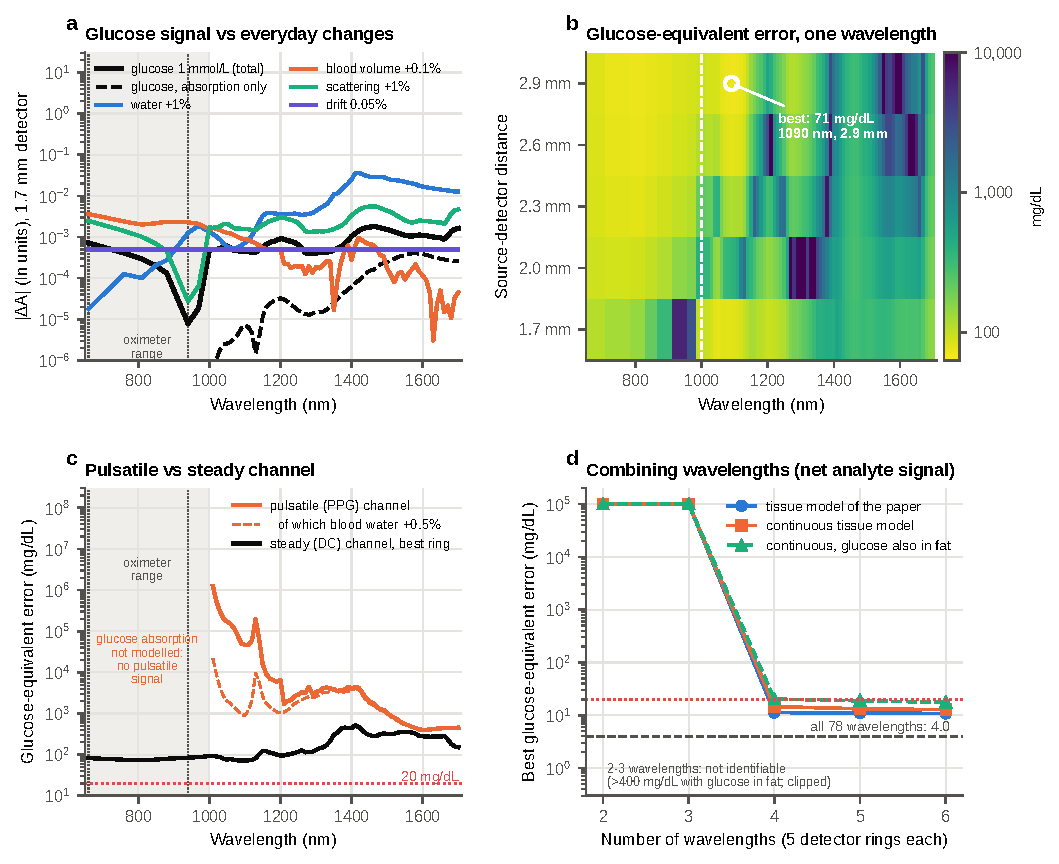
\includegraphics[width=\linewidth]{figs/fig4_simulation.pdf}
\caption{Monte Carlo analysis of three-layer skin, 660 to 1700~nm. The grey band marks the pulse-oximeter range (dotted lines at 660 and 940~nm), where tissue properties come from a composition model and glucose acts only through scattering. (a) Absorbance change at the 1.7~mm detector for 1~mmol/L of glucose and for typical non-glucose changes. (b) Glucose-equivalent error of all confounders combined (root sum of squares) for every wavelength and detector distance; the best single channel is 71~\mgdl{} at 1090~nm and 2.9~mm. (c) Best achievable error for the pulsatile (PPG) channel and for the steady (DC) channel; below 1000~nm glucose absorption is not modelled, so the pulsatile channel carries no glucose signal there by construction. (d) Best error when wavelengths are combined, using all five detector rings per wavelength (net analyte signal, 0.05\% noise per channel, wavelengths at least 30~nm apart), for the main tissue model and for the continuous alternative model with and without glucose in the fat layer. Two wavelengths, and three in the main and continuous models, cannot separate glucose from the confounders (errors above $10^{13}$~\mgdl{}, numerically non-identifiable); with glucose also in the fat layer, three wavelengths give finite but very large errors (above 400~\mgdl{}; Table~S6), so no useful estimate. Values above the plotted range are clipped.}
\label{fig:sim}
\end{figure}

\begin{table}[!htbp]
\centering\small
\begin{threeparttable}
\caption{Simulation summary: best glucose-equivalent error (\mgdl{}) for each sensing configuration, 660 to 1700~nm (78 wavelengths, 5 detectors).}
\label{tab:sim}
\begin{tabular}{@{}lr@{}}
\toprule
Configuration & Error (\mgdl{}) \\
\midrule
\multicolumn{2}{@{}l}{\emph{Single wavelength, steady (DC) channel}} \\
Best overall (1090~nm, 2.9~mm) & 71 \\
\quad of which: scattering $+1\%$ / blood volume $+0.1\%$ / water $+1\%$ / drift 0.05\% & 61 / 29 / 20 / 11 \\
Oximeter wavelengths, best detector: 660 / 940~nm\tnote{a} & 82 / 84 \\
If glucose acted through absorption only (1600~nm, 2.3~mm) & 790 \\
Glucose scattering coefficient $\times0.5$ / $\times2$ & 141 / 36 \\
Photon shot noise alone (5~mW source, 10~s), any channel & $<3$ \\
\multicolumn{2}{@{}l}{\emph{Single wavelength, pulsatile (PPG) channel}} \\
660 to 970~nm (glucose absorption not modelled) & no signal \\
Best wavelength (1600~nm)\tnote{b} & 400 \\
\multicolumn{2}{@{}l}{\emph{Several wavelengths, all five detectors (net analyte signal)}} \\
Two or three wavelengths & $>10^{13}$ \\
Four (1340, 1420, 1580, 1620~nm) & 11 \\
Five (adds 1660~nm) & 11 \\
Six (adds 1150~nm) & 11 \\
All 78 wavelengths (idealised bound) & 4.0 \\
\bottomrule
\end{tabular}
\begin{tablenotes}\footnotesize
\item[a] Entirely through the assumed glucose scattering coefficient, which is not specific to glucose. \item[b] 400 to 550~\mgdl{} over 1550 to 1700~nm; dominated by a 0.5\% change in blood water content. Multi-wavelength rows: best sets of wavelengths at least 30~nm apart; glucose absorption alone gives the same errors, because the scattering part of the glucose signal is removed together with the scattering confounder.
\end{tablenotes}
\end{threeparttable}
\end{table}

At the best single channel (1090~nm, 2.9~mm), the confounders combined correspond to 71~\mgdl{} (Figure~\ref{fig:sim}b, Table~\ref{tab:sim}). This figure depends directly on the assumed glucose scattering coefficient: halving it doubles the error, and without any scattering effect the best single channel is 790~\mgdl{}. Photon shot noise is negligible ($<3$~\mgdl{} in every channel), so the limit is physiology and drift, not the detector.

The pulsatile channel, which is what a PPG measures, is worse than the steady channel at every wavelength above 1000~nm (Figure~\ref{fig:sim}c): the arterial blood volume is small and its water content dominates the pulse, so a 0.5\% change in blood water alone corresponds to 400 to 550~\mgdl{} at 1550 to 1700~nm.

Combining wavelengths helps only when there are enough of them (Figure~\ref{fig:sim}d). With five detector rings per wavelength, no pair or triple of wavelengths can separate glucose from water, blood volume, scattering and drift. Four wavelengths can: the best set at least 30~nm apart (1340, 1420, 1580 and 1620~nm) reaches 11~\mgdl{} under the idealised linear model, and a fifth or sixth wavelength adds little (11.0 and 10.9~\mgdl{}). The glucose scattering effect points in the same direction as any other change in dermal scattering, so the net-analyte analysis removes it entirely: glucose absorption alone gives exactly the same multi-wavelength errors, the selectivity is 0.57 for glucose absorption alone and 0.14 when scattering is included, and with all 78 wavelengths both reach the same idealised bound of 4.0~\mgdl{}. In other words, only glucose absorption is specific, and separating it requires spectral diversity rather than more detector spacings.

\textbf{Why four wavelengths.} The wavelength count follows from the structure of the sensitivity matrix rather than from the noise level. All modelled absorbers (water, blood volume, oxygen saturation and glucose) sit in the dermis, so at a given wavelength their effects on the five detectors are proportional to the same partial-pathlength profile and can be told apart only by their spectra; scattering changes and an offset add two more directions. Stacking the confounder columns $K$ and the glucose vector $g$ over the selected channels, the rank of $[K\;g]$ equals the rank of $K$ for two and three wavelengths (4 and 5): the glucose vector lies inside the confounder space and no linear combination of channels can isolate it (condition number of $[K\;g]$ above $10^{16}$). With four wavelengths the rank of $[K\;g]$ rises to 6, one more than that of $K$ (condition number 537 for the best set; 349 and 214 with five and six wavelengths). Propagating the Monte Carlo standard errors of the sensitivities changes the errors by less than 1\% (11.3, 95\% interval 11.3 to 11.4~\mgdl{}, for four wavelengths), and requiring 50~nm instead of 30~nm between wavelengths changes them by less than 0.5~\mgdl{}. These intervals reflect photon statistics only; the tissue model was varied separately (below), the confounder set was not. The conclusion is therefore conditional: under the modelled tissue properties, confounders and noise, single-wavelength measurements carry large glucose-equivalent uncertainty and glucose becomes identifiable only with at least as many wavelengths as there are absorbing components. This is not a minimum wavelength count for a real device; establishing one would require broader sensitivity analyses (tissue properties, geometry, confounder set and noise model) or experimental data.

\textbf{Pulse-oximeter wavelengths.} At 660 and 940~nm, the wavelengths of the VitalDB oximeters, the steady channel reaches 82 and 84~\mgdl{} at best, similar to the near infrared, but only through the assumed glucose scattering effect, which any other change in dermal scattering mimics (Table~\ref{tab:sim}). Glucose absorption was not modelled below 1000~nm, so in the model the pulsatile channel, the signal a PPG records, has no glucose-specific component there; this follows from the assumption and is not a result of the simulation. Glucose does absorb weakly near 910, 960 and 985~nm, and these bands change with temperature in the same way as with sugar concentration~\citep{golic2003}; their contribution to a 660/940~nm PPG remains unresolved by the present model. Within the model, a 660/940~nm PPG can respond to glucose only indirectly, through scattering or haemodynamic changes that accompany it. When a small glucose absorption is assumed below 1000~nm (alternative model, below), the pulsatile channel still needs a glucose-equivalent error above $10^5$~\mgdl{} there.

\textbf{Sensitivity to the tissue model.} The continuous alternative model (Section~\ref{sec:simmethods}) leads to the same conclusions (Table~S6). The best single channel is 73~\mgdl{} (720~nm, 2.9~mm; 74~\mgdl{} at 1090~nm) against 71~\mgdl{}, the oximeter wavelengths reach 87 and 91~\mgdl{}, glucose absorption alone still needs 790~\mgdl{}, two wavelengths still cannot separate glucose, three cannot in this model and give errors above 400 to 1,000~\mgdl{} (finite but of no practical use) when glucose also acts in the fat, and four well-chosen wavelengths reach 15~\mgdl{} (13 with six). Letting glucose also act in the subcutaneous fat changes the single-channel errors to 68 to 136~\mgdl{} and the four-wavelength error to 18 to 20~\mgdl{}, depending on how strongly the fat contributes, because the fat layer brings its own water, blood and scattering confounders. The quantitative values therefore depend on the tissue optics and on where glucose acts (by up to about 60\% at the oximeter wavelengths), but none of the qualitative conclusions does: no single wavelength reaches clinically useful accuracy, the pulse at oximeter wavelengths carries no usable glucose signal, and separation needs several near-infrared wavelengths.


\FloatBarrier
\subsection{Device model}
\label{sec:device}
The deployed model uses only inputs a wearable has. Trained and evaluated on features computed exactly as on the device from the minute of PPG before each reading (person-level 5-fold), the calibration-free model reaches RMSE 33.3~\mgdl{} (\RR{} 0.130) against 34.2~\mgdl{} (\RR{} 0.082) for the profile alone (Table~\ref{tab:device}). With one reference value, RMSE is 30.9~\mgdl{} against 32.3~\mgdl{} for the same model without PPG, a PPG gain of 1.42~\mgdl{} (95\% CI 0.56 to 2.35). This gain is encouraging but sensitive to window selection: with a 60-s window centred on the recorded sample time instead of the minute before it, the calibrated model reaches 31.8~\mgdl{} and the gain, 0.47~\mgdl{} ($-0.65$ to 1.55), is not significant. The device's PPG contribution is therefore of the same small size as in the full analysis (Sections~\ref{sec:leak} to \ref{sec:subgroups}) and depends on which minute is used.

A running mean of the features over several minutes costs nothing on the device, so we tested averaging the last 3, 5 and 10~min before the reading, and, retrospectively, the whole 16-min recording. None improved on a single minute beyond its confidence interval (Table~\ref{tab:device}), so the firmware estimates from the latest minute; the running mean remains a compile-time option.

\begin{table}[!htbp]
\centering\footnotesize\setlength{\tabcolsep}{3.2pt}
\begin{threeparttable}
\caption{Device model (15 PPG features + age, sex, BMI, diabetes), person-level 5-fold, by PPG window. Upper block: features from, or averaged over, the last $K$ one-minute windows before the recorded sample time (usable in real time), plus a retrospective comparison over the whole 16-min recording. Lower block: a 60-s window centred on the recorded time (also retrospective).}
\label{tab:device}
\begin{tabular}{@{}lcccc@{}}
\toprule
& \multicolumn{2}{c}{Calibration-free} & \multicolumn{2}{c}{One reference value} \\
\cmidrule(lr){2-3}\cmidrule(l){4-5}
PPG window & RMSE (\mgdl{}) & \RR{} & RMSE (\mgdl{}) & PPG gain (95\% CI) \\
\midrule
No PPG features & 34.2 & 0.082 & 32.3 & -- \\
\rowcolor{rowgray} Last 1 min (deployed) & 33.3 & 0.130 & 30.9 & $-1.42$ ($-2.35$, $-0.56$) \\
Mean of last 3 min & 33.3 & 0.130 & 31.1 & $-1.26$ ($-2.05$, $-0.57$) \\
Mean of last 5 min & 33.3 & 0.131 & 31.4 & $-0.94$ ($-1.86$, $-0.18$) \\
Mean of last 10 min & 33.4 & 0.127 & 31.0 & $-1.33$ ($-2.10$, $-0.61$) \\
All 16 min, retrospective\tnote{a} & 33.2 & 0.135 & 31.2 & $-1.10$ ($-2.07$, $-0.23$) \\
\midrule
60 s centred on the recorded time & 33.4 & 0.128 & 31.8 & $-0.47$ ($-1.55$, $+0.65$) \\
\bottomrule
\end{tabular}
\begin{tablenotes}\footnotesize
\item All calibrated rows use the same calibration pairs (4,034 later readings from the same recording session as the calibration). PPG gain: paired change in RMSE against the calibrated model without PPG (32.31~\mgdl{}); 500 patient-bootstrap resamples.
\item[a] Retrospective comparison: includes the 8~min after the recorded sample time, so not usable in real time.
\end{tablenotes}
\end{threeparttable}
\end{table}

\subsection{ESP32-S3 performance}
\label{sec:esp}
The firmware and both tree models occupy 945~kB of flash (31\% of a 3~MB application partition) and leave 80~kB of heap free (Table~S7). One 60-s window takes 311~ms in the boot self-test: 275~ms for filtering and beat extraction, 33~ms for the 15 features and 3~ms for the 300 trees. The per-beat TinyCNN takes 1,555~ms on the same window, 15~ms per beat (Figure~\ref{fig:embedded}a). The original ResNet34 implementation on an STM32H743 reported an inference time of 6.4~s~\citep{zeynali2025}; it is shown for scale only: it was obtained with a different model, workload and microcontroller, so the two times are not a speed comparison.

In the hardware-in-the-loop test every estimate from the board was identical to the Python reference for all 30 tested recordings, with a maximum difference of 0~\mgdl{} for both models (Figure~\ref{fig:embedded}b). The median processing time was 304~ms per one-minute window (range 253 to 340~ms). Bit-for-bit agreement required NumPy's pairwise summation in the firmware: with ordinary sequential sums, one of the 30 test cases crossed a tree threshold because of a $10^{-13}$ difference in one feature, and its estimate differed by 0.16~\mgdl{}.


\begin{figure}[!htbp]
\centering
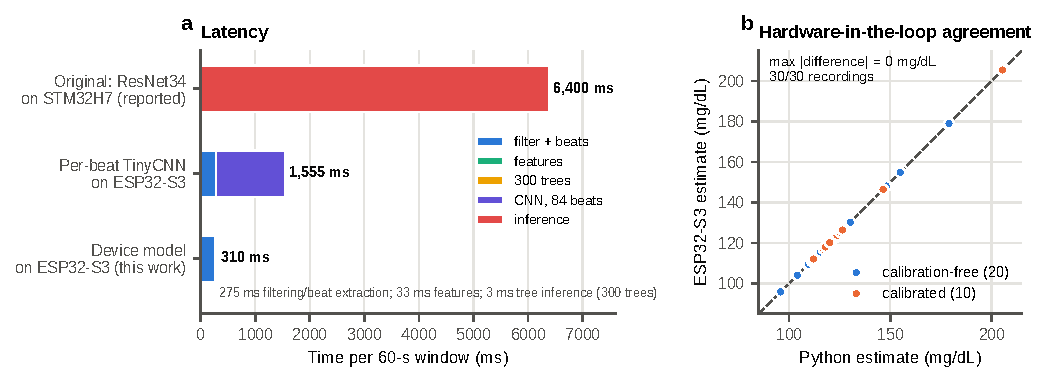
\includegraphics[width=\linewidth]{figs/fig5_embedded.pdf}
\caption{(a) Processing time for one 60-s window on the ESP32-S3 for the device model and the per-beat TinyCNN, with the inference time reported for the original STM32H7 implementation~\citep{zeynali2025} for scale only (different model, workload and hardware; not a speed comparison). (b) Glucose estimates of the ESP32-S3 against the Python reference in the hardware-in-the-loop test (30 VitalDB recordings); all points lie on the identity line.}
\label{fig:embedded}
\end{figure}

\FloatBarrier
% =====================================================================
\section{Discussion}
Clinical PPG at oximeter wavelengths carries little person-independent glucose information. Accuracy measured with segment-level splits mainly reflects performance on patients already seen in training; for new patients, what remains is modest, real, and explained by context rather than by a glucose-specific optical signal.

Table~\ref{tab:summary} groups the person-level results by the information a device would have, because the best overall numbers rely on operating-room data that no wearable has.

\begin{table}[!htbp]
\centering\footnotesize\setlength{\tabcolsep}{3.5pt}
\begin{threeparttable}
\caption{Person-level results grouped by available inputs (VitalDB, 5-fold by patient).}
\label{tab:summary}
\begin{tabular}{@{}llccc@{}}
\toprule
Inputs available & Model & RMSE (\mgdl{}) & \RR{} & Reference without PPG \\
\midrule
\multicolumn{5}{@{}l}{\emph{1. PPG alone}} \\
& PPG features (GBM) & 35.1 & 0.034 & training mean: 35.7 \\
& ResNet34-1D & 35.0 & 0.042 & \\
& Device features, 60~s centred & 35.6 & 0.009 & \\
\multicolumn{5}{@{}l}{\emph{2. PPG + demographics or one calibration value (wearable inputs)}} \\
& Multi-beat CNN + age, sex, BMI & 33.8 & 0.102 & age, sex, BMI: 35.0 \\
& Pretrained Pulse-PPG + age, sex, BMI & 34.0 & 0.097 & \\
& Device model + profile & 33.3 & 0.130 & profile only: 34.2 \\
& Device model + profile + calibration\tnote{a} & 30.9 & -- & same without PPG: 32.3 \\
\multicolumn{5}{@{}l}{\emph{3. PPG + operating-room context}} \\
& Clinical + time + PPG & 31.8 & 0.207 & clinical + time: 32.9 \\
& All signals & 31.3 & 0.233 & -- \\
& All signals + calibration\tnote{b} & 30.8 & 0.325 & calibration + clinical + time: 33.0 \\
\bottomrule
\end{tabular}
\begin{tablenotes}\footnotesize
\item[a] 4,034 readings from the same session as the calibration; features from the minute before each reading (with a centred minute: 31.8, PPG gain not significant; Table~\ref{tab:device}). \item[b] 4,233 readings scored after each patient's first.
\end{tablenotes}
\end{threeparttable}
\end{table}

\textbf{Why the split matters.} The same ResNet34-1D, data and training moved between \RR{} 0.23 and 0.04 only by changing how segments were split. Adjacent beats from one reading are near-duplicates, so a segment-level test set mostly measures performance on known patients. Ramesh et al.~\citep{ramesh2026} reached the same conclusion independently by reimplementing published models (\RR{} 0.60 under random splits, below zero under participant-aware splits for our model). Our results add the size of the effect on a 2,991-patient cohort with patient-level confidence intervals, the evidence that Clarke A+B does not reflect it, and the MUST transfer test, in which no model beat a constant prediction.

\textbf{What PPG does add.} Under person-level evaluation the PPG features still lower the error significantly: by 1.1~\mgdl{} over clinical context and time, and by 1.4 to 1.7~\mgdl{} when one reference reading per person is available (less robustly for the wearable-input device model; Section~\ref{sec:device}). Gains of this size are statistically clear but clinically small (RMSE 31 against a 36~\mgdl{} spread), and the subgroup analysis shows where they fall short: no model detects hypoglycaemia usefully (at best 2 of 58 readings, sensitivity 3.4\%), and high values are underestimated by 44~\mgdl{} or more even after calibration (Section~\ref{sec:subgroups}). They are consistent with PPG tracking haemodynamic state (vascular tone, perfusion and heart rate~\citep{allen2007}) that correlates with glucose during surgery, rather than glucose itself. Adding ECG, arterial pressure and monitor numerics brought no further significant gain, and conversely PPG adds nothing once those signals are present (Table~\ref{tab:logo}): they carry largely the same information, consistent with a predominantly haemodynamic origin. For a wearable this cuts both ways: PPG alone captures most of what the bedside haemodynamic signals offer, but that information is not glucose-specific. The gain is not an artefact of look-ahead, since PPG recorded only before the draw gives the same result (Table~S3).

\textbf{Model capacity was not the limiting factor here.} Person-level \RR{} stayed between 0.04 and 0.10 for every PPG model we evaluated: a 12-k-parameter TinyCNN, the 7.4-M-parameter ResNet34-1D, a multi-beat CNN, and two foundation models with 5 to 28~M parameters pretrained on up to 57,641~h of PPG, including VitalDB itself (Section~\ref{sec:fm}). Fine-tuning did not reduce the validation error, and with clinical context the pretrained embeddings were interchangeable with 17 hand-crafted features. When encoders of such different size, architecture and pretraining converge on the accuracy of simple features, the limit for these data appears to lie in the information the signal carries about glucose in people not seen in training rather than in model capacity. This does not exclude that other architectures, inputs or training data could extract more.

\textbf{How the data and the simulation relate.} The two lines of evidence are consistent, but they do not establish the same mechanism: the data show how much person-independent information clinical PPG carries, and the simulation shows what the modelled optics allow. Under its assumptions, the simulation shows that a single-wavelength reflectance signal cannot separate glucose from normal changes in water, blood volume and dermal scattering: the best case is a model-derived glucose-equivalent error of 71~\mgdl{} (not a measured prediction error), and 790~\mgdl{} when only glucose absorption is counted. Glucose's scattering effect is real but not specific, because any change in dermal scattering produces the same signature. The pulsatile channel, which is what a PPG measures, is worse than the steady channel, because the arterial blood volume is small and its water content dominates. At the oximeter wavelengths glucose absorption was not modelled, so the simulation cannot rule out a weak direct contribution there; it does show that any such contribution must compete with much larger scattering and haemodynamic changes. Because the weak glucose bands near 910 to 985~nm are not resolved in either tissue model, the simulation constrains but does not settle the question for 660/940~nm PPG; that a network trained on such PPG reaches glucose mainly through indirect correlates is consistent with, but not proven by, what we measured.

\textbf{A realistic route.} Within the modelled tissue and confounder set, the simulation indicates that at least four well-separated near-infrared wavelengths are needed (a model-dependent identifiability result, not a general requirement for optical glucose sensors), measured on the steady channel with several detector spacings, together with InGaAs detection and per-person calibration. Under idealised conditions four such wavelengths reach about 11 to 20~\mgdl{} depending on the tissue model, and more wavelengths add little. The embedded results show that the computing side is not the obstacle: feature extraction plus a 300-tree model runs in about 0.3~s on a low-cost microcontroller, with results identical to the PC on all tested recordings.

\textbf{Limitations.}
\begin{itemize}[leftmargin=*]
\item VitalDB patients are anaesthetised, fasting and haemodynamically managed~\citep{lee2022vitaldb}. Performance in daily life may differ in either direction, and the gains from clinical context (time since anaesthesia, drugs) do not transfer outside the operating room.
\item Glucose labels are intermittent laboratory values, assumed constant for $\pm$8~min around the recorded time, which may differ from the actual blood draw by an unknown amount; this affects the causal analysis as well as the label itself. Hypoglycaemia is rare in this cohort (102 readings below 70~\mgdl{}), so performance in that range is estimated from few patients.
\item The 1-s single-peak window rejects beats above about 120~bpm.
\item MUST is small (23 people, 10-s recordings) and was recorded with a different sensor and wavelength.
\item The ESP32 test recordings were part of the final model's training data; the test verifies numerical fidelity, not accuracy, and a prospective wearable study is still required.
\item The simulation models reflectance from skin with detectors 1.7 to 2.9~mm from the source, whereas the VitalDB oximeters measure transmission through the fingertip. The pulsatile-channel argument depends only on the absorption of glucose relative to blood and is independent of geometry, but the absolute steady-channel errors apply to the modelled geometry.
\item The optical model is first-order. It omits temperature-dependent water absorption, variation in skin thickness and melanin, and contact pressure; tissue optics were varied only between two models. The glucose scattering coefficient comes from one human study~\citep{ge2024}, and its fractional value is assumed constant over wavelength. The net-analyte errors assume an ideal linear calibration and are therefore lower bounds. Below 1000~nm the tissue properties of the main model come from a composition model rather than from one measured data set, and glucose absorption there is set to zero; the step at 1000~nm in Figure~\ref{fig:sim} reflects this change of data source. A continuous alternative model without this step, and with a small glucose absorption below 1000~nm, gave the same conclusions (Table~S6), but both models share the same geometry and confounder set. Glucose absorption below 1000~nm is known only at two wavelengths and the weak bands near 910 to 985~nm are not resolved; the measured scattering peak at 1450~nm was smoothed, not modelled.
\end{itemize}

\section{Conclusion}
Evaluated person by person, deep-learning PPG glucose estimation from clinical oximeters performs close to demographics alone (\RR{} 0.04 to 0.10 rather than the 0.23 seen with random splits), also with pretrained PPG foundation models, and it does not transfer to an independent dataset. Combined with clinical context and one calibration reading, the change in PPG features gives a small but significant improvement on the same readings (RMSE 33.0 to 31.3~\mgdl{}). Monte Carlo modelling is consistent with this: under the modelled tissue properties and confounders, physiological variation masks glucose at any single wavelength, and glucose becomes identifiable only with four or more near-infrared wavelengths, a property of the modelled sensitivity matrix rather than a validated design rule for a device. None of the models evaluated here is suitable for clinical glucose monitoring: they detect at most 3.4\% of hypoglycaemic readings and underestimate high values. The wearable-input gradient-boosting pipeline, evaluated with patient-independent cross-validation, was implemented on the ESP32-S3 and processed a 60-s PPG recording in about 0.3~s, with numerical agreement on all 30 hardware test recordings, so the remaining work for non-invasive glucose sensing lies in optics, calibration and prospective validation, not computation.

\section*{Data and code availability}
VitalDB is openly available at \url{https://vitaldb.net}~\citep{lee2022vitaldb} and MUST on Mendeley Data~\citep{must2023}. All code needed to reproduce the results, from data download and fold assignment to the Monte Carlo analyses and the ESP32 firmware, is available at \url{https://github.com/arash1602/ppg-glucose-reassessment} (release v1.0); the Monte Carlo framework it builds on is at \url{https://github.com/milanbhutan/Glucose_Sensor_Ranking}.

\section*{Ethics statement}
This study used only two public, de-identified datasets (VitalDB and MUST), released by their custodians for research with ethical approval and consent obtained at collection~\citep{lee2022vitaldb,must2023}. No new data were collected from people, and the analysis involved no interaction with participants and no access to identifiable information.

\section*{Funding}
This work was supported by the Lockheed Martin Endowed Professorship awarded to M.~Ghamari by the College of Engineering, California Polytechnic State University, San Luis Obispo, for the project ``Advancing Diabetes Care: A Non-Invasive Blood Glucose Monitoring System Powered by Embedded AI''. The funder had no role in study design, data analysis, decision to publish or preparation of the manuscript.

\section*{CRediT authorship contribution statement}
\textbf{Mohammad Ghamari:} Conceptualization, Methodology, Software, Formal analysis, Investigation, Visualization, Writing -- original draft, Writing -- review \& editing, Supervision, Funding acquisition. \textbf{Milan Chhetri:} Methodology, Software (Monte Carlo skin model), Formal analysis (optical simulation), Writing -- review \& editing. \textbf{Souvik Kundu:} Writing -- review \& editing. \textbf{Khalil Alipour:} Writing -- review \& editing. \textbf{Bahram Tarvirdizadeh:} Writing -- review \& editing.

\section*{Declaration of competing interest}
The authors declare that they have no known competing financial interests or personal relationships that could have appeared to influence the work reported in this paper. M.~Ghamari, K.~Alipour and B.~Tarvirdizadeh are co-authors of the previous study re-evaluated here~\citep{zeynali2025}.

\begin{thebibliography}{99}\small
\setlength{\itemsep}{1pt}
\bibitem{allen2007} Allen J. Photoplethysmography and its application in clinical physiological measurement. \emph{Physiol Meas}. 2007;28(3):R1--R39. doi:10.1088/0967-3334/28/3/R01.
\bibitem{castaneda2018} Castaneda D, Esparza A, Ghamari M, Soltanpur C, Nazeran H. A review on wearable photoplethysmography sensors and their potential future applications in health care. \emph{Int J Biosens Bioelectron}. 2018;4(4):195. doi:10.15406/ijbsbe.2018.04.00125.
\bibitem{montemoreno2011} Monte-Moreno E. Non-invasive estimate of blood glucose and blood pressure from a photoplethysmograph by means of machine learning techniques. \emph{Artif Intell Med}. 2011;53(2):127--138. doi:10.1016/j.artmed.2011.05.001.
\bibitem{chu2021} Chu J, Yang W-T, Lu W-R, Chang Y-T, Hsieh T-H, Yang F-L. 90\% accuracy for photoplethysmography-based non-invasive blood glucose prediction by deep learning with cohort arrangement and quarterly measured HbA1c. \emph{Sensors}. 2021;21(23):7815. doi:10.3390/s21237815.
\bibitem{gupta2021} Gupta SS, Kwon T-H, Hossain S, Kim K-D. Towards non-invasive blood glucose measurement using machine learning: an all-purpose PPG system design. \emph{Biomed Signal Process Control}. 2021;68:102706.
\bibitem{prabha2022} Prabha A, Yadav J, Rani A, Singh V. Intelligent estimation of blood glucose level using wristband PPG signal and physiological parameters. \emph{Biomed Signal Process Control}. 2022;78:103876.
\bibitem{zeynali2025} Zeynali M, Alipour K, Tarvirdizadeh B, Ghamari M. Non-invasive blood glucose monitoring using PPG signals with various deep learning models and implementation using TinyML. \emph{Sci Rep}. 2025;15:581. doi:10.1038/s41598-024-84265-8.
\bibitem{lee2022vitaldb} Lee H-C, Park Y, Yoon SB, Yang SM, Park D, Jung C-W. VitalDB, a high-fidelity multi-parameter vital signs database in surgical patients. \emph{Sci Data}. 2022;9:279. doi:10.1038/s41597-022-01411-5.
\bibitem{amerov2004} Amerov AK, Chen J, Arnold MA. Molar absorptivities of glucose and other biological molecules in aqueous solutions over the first overtone and combination regions of the near-infrared spectrum. \emph{Appl Spectrosc}. 2004;58(10):1195--1204. doi:10.1366/0003702042336136.
\bibitem{jubran2015} Jubran A. Pulse oximetry. \emph{Crit Care}. 2015;19:272. doi:10.1186/s13054-015-0984-8.
\bibitem{golic2003} Golic M, Walsh K, Lawson P. Short-wavelength near-infrared spectra of sucrose, glucose, and fructose with respect to sugar concentration and temperature. \emph{Appl Spectrosc}. 2003;57(2):139--145.
\bibitem{kohl1994} Kohl M, Cope M, Essenpreis M, B\"ocker D. Influence of glucose concentration on light scattering in tissue-simulating phantoms. \emph{Opt Lett}. 1994;19(24):2170--2172.
\bibitem{larin2003} Larin KV, Motamedi M, Ashitkov TV, Esenaliev RO. Specificity of noninvasive blood glucose sensing using optical coherence tomography technique: a pilot study. \emph{Phys Med Biol}. 2003;48(10):1371--1390. doi:10.1088/0031-9155/48/10/310.
\bibitem{saeb2017} Saeb S, Lonini L, Jayaraman A, Mohr DC, Kording KP. The need to approximate the use-case in clinical machine learning. \emph{GigaScience}. 2017;6(5):gix019. doi:10.1093/gigascience/gix019.
\bibitem{kapoor2023} Kapoor S, Narayanan A. Leakage and the reproducibility crisis in machine-learning-based science. \emph{Patterns}. 2023;4(9):100804. doi:10.1016/j.patter.2023.100804.
\bibitem{ramesh2026} Ramesh S, Neufeld M, K\"uttner M, R\"oddiger T, Beigl M. Reassessing the feasibility of PPG-based non-invasive blood glucose level estimation. In: \emph{Proc 2026 ACM International Symposium on Wearable Computers (ISWC '26)}. ACM; 2026. p.~127--133. doi:10.1145/3830727.3834821.
\bibitem{hammour2023} Hammour G, Mandic DP. An in-ear PPG-based blood glucose monitor: a proof-of-concept study. \emph{Sensors}. 2023;23(6):3319. doi:10.3390/s23063319.
\bibitem{must2023} Kermani A, Esmaeili H. The dataset of photoplethysmography signals collected from a pulse sensor to measure blood glucose level. Mendeley Data, version 1; 2023. doi:10.17632/37pm7jk7jn.1.
\bibitem{he2016} He K, Zhang X, Ren S, Sun J. Deep residual learning for image recognition. In: \emph{Proc IEEE Conf Computer Vision and Pattern Recognition (CVPR)}; 2016. p.~770--778.
\bibitem{zaheer2017} Zaheer M, Kottur S, Ravanbakhsh S, P\'oczos B, Salakhutdinov R, Smola AJ. Deep sets. In: \emph{Advances in Neural Information Processing Systems 30}; 2017. p. 3391--3401.
\bibitem{paszke2019} Paszke A, Gross S, Massa F, et al. PyTorch: an imperative style, high-performance deep learning library. In: \emph{Advances in Neural Information Processing Systems 32}; 2019. p.~8024--8035.
\bibitem{loshchilov2019} Loshchilov I, Hutter F. Decoupled weight decay regularization. In: \emph{International Conference on Learning Representations (ICLR)}; 2019.
\bibitem{pillai2025} Pillai A, Spathis D, Kawsar F, Malekzadeh M. PaPaGei: open foundation models for optical physiological signals. In: \emph{International Conference on Learning Representations (ICLR)}; 2025.
\bibitem{saha2025} Saha M, Xu MA, Mao W, Neupane S, Rehg JM, Kumar S. Pulse-PPG: an open-source field-trained PPG foundation model for wearable applications across lab and field settings. \emph{Proc ACM Interact Mob Wearable Ubiquitous Technol}. 2025;9(3):1--35. doi:10.1145/3749494.
\bibitem{friedman2001} Friedman JH. Greedy function approximation: a gradient boosting machine. \emph{Ann Stat}. 2001;29(5):1189--1232. doi:10.1214/aos/1013203451.
\bibitem{pedregosa2011} Pedregosa F, Varoquaux G, Gramfort A, et al. Scikit-learn: machine learning in Python. \emph{J Mach Learn Res}. 2011;12:2825--2830.
\bibitem{elgendi2012} Elgendi M. On the analysis of fingertip photoplethysmogram signals. \emph{Curr Cardiol Rev}. 2012;8(1):14--25. doi:10.2174/157340312801215782.
\bibitem{elgendi2016} Elgendi M. Optimal signal quality index for photoplethysmogram signals. \emph{Bioengineering}. 2016;3(4):21. doi:10.3390/bioengineering3040021.
\bibitem{duggan2017} Duggan EW, Carlson K, Umpierrez GE. Perioperative hyperglycemia management: an update. \emph{Anesthesiology}. 2017;126(3):547--560. doi:10.1097/ALN.0000000000001515.
\bibitem{taskforce1996} Task Force of the European Society of Cardiology and the North American Society of Pacing and Electrophysiology. Heart rate variability: standards of measurement, physiological interpretation and clinical use. \emph{Circulation}. 1996;93(5):1043--1065. doi:10.1161/01.CIR.93.5.1043.
\bibitem{mukkamala2015} Mukkamala R, Hahn J-O, Inan OT, Mestha LK, Kim C-S, T\"oreyin H, Kyal S. Toward ubiquitous blood pressure monitoring via pulse transit time: theory and practice. \emph{IEEE Trans Biomed Eng}. 2015;62(8):1879--1901. doi:10.1109/TBME.2015.2441951.
\bibitem{clarke1987} Clarke WL, Cox D, Gonder-Frederick LA, Carter W, Pohl SL. Evaluating clinical accuracy of systems for self-monitoring of blood glucose. \emph{Diabetes Care}. 1987;10(5):622--628.
\bibitem{efron1993} Efron B, Tibshirani RJ. \emph{An Introduction to the Bootstrap}. New York: Chapman \& Hall; 1993.
\bibitem{fang2009} Fang Q, Boas DA. Monte Carlo simulation of photon migration in 3D turbid media accelerated by graphics processing units. \emph{Opt Express}. 2009;17(22):20178--20190. doi:10.1364/OE.17.020178.
\bibitem{ge2024} Ge Q, Han T, Liu R, Zhang Z, Sun D, Liu J, Xu K. Evaluation and validation on sensitivity of near-infrared diffuse reflectance in non-invasive human blood glucose measurement. \emph{Sensors}. 2024;24(18):5879. doi:10.3390/s24185879.
\bibitem{iino2003} Iino K, Maruo K, Arimoto H, Hyodo K, Nakatani T, Yamada Y. Monte Carlo simulation of near infrared reflectance spectroscopy in the wavelength range from 1000~nm to 1900~nm. \emph{Opt Rev}. 2003;10(6):600--606.
\bibitem{bosschaart2014} Bosschaart N, Edelman GJ, Aalders MCG, van Leeuwen TG, Faber DJ. A literature review and novel theoretical approach on the optical properties of whole blood. \emph{Lasers Med Sci}. 2014;29(2):453--479. doi:10.1007/s10103-013-1446-7.
\bibitem{simpson1998} Simpson CR, Kohl M, Essenpreis M, Cope M. Near-infrared optical properties of ex vivo human skin and subcutaneous tissues measured using the Monte Carlo inversion technique. \emph{Phys Med Biol}. 1998;43(9):2465--2478. doi:10.1088/0031-9155/43/9/003.
\bibitem{shimojo2020} Shimojo Y, Nishimura T, Hazama H, Ozawa T, Awazu K. Measurement of absorption and reduced scattering coefficients in Asian human epidermis, dermis, and subcutaneous fat tissues in the 400- to 1100-nm wavelength range for optical penetration depth and energy deposition analysis. \emph{J Biomed Opt}. 2020;25(4):045002. doi:10.1117/1.JBO.25.4.045002.
\bibitem{jacques2013} Jacques SL. Optical properties of biological tissues: a review. \emph{Phys Med Biol}. 2013;58(11):R37--R61. doi:10.1088/0031-9155/58/11/R37.
\bibitem{segelstein1981} Segelstein DJ. \emph{The complex refractive index of water}. MSc thesis, University of Missouri--Kansas City; 1981.
\bibitem{hale1973} Hale GM, Querry MR. Optical constants of water in the 200-nm to 200-$\mu$m wavelength region. \emph{Appl Opt}. 1973;12(3):555--563. doi:10.1364/AO.12.000555.
\bibitem{kou1993} Kou L, Labrie D, Chylek P. Refractive indices of water and ice in the 0.65- to 2.5-$\mu$m spectral range. \emph{Appl Opt}. 1993;32(19):3531--3540. doi:10.1364/AO.32.003531.
\bibitem{ganesan2016} Ganesan G, Warren RV, Leproux A, Compton M, Cutler K, Wittkopp S, Tran G, O'Sullivan T, Malik S, Galassetti PR, Tromberg BJ. Diffuse optical spectroscopic imaging of subcutaneous adipose tissue metabolic changes during weight loss. \emph{Int J Obes}. 2016;40(8):1292--1300. doi:10.1038/ijo.2016.43.
\bibitem{salomatina2006} Salomatina E, Jiang B, Novak J, Yaroslavsky AN. Optical properties of normal and cancerous human skin in the visible and near-infrared spectral range. \emph{J Biomed Opt}. 2006;11(6):064026. doi:10.1117/1.2398928.
\bibitem{vangemert1989} van Gemert MJC, Jacques SL, Sterenborg HJCM, Star WM. Skin optics. \emph{IEEE Trans Biomed Eng}. 1989;36(12):1146--1154. doi:10.1109/10.42108.
\bibitem{haque2021} Haque CA, Hossain S, Kwon T-H, Kim K-D. Noninvasive in vivo estimation of blood-glucose concentration by Monte Carlo simulation. \emph{Sensors}. 2021;21(14):4918. doi:10.3390/s21144918.
\bibitem{hayakawa2001} Hayakawa CK, Spanier J, Bevilacqua F, Dunn AK, You JS, Tromberg BJ, Venugopalan V. Perturbation Monte Carlo methods to solve inverse photon migration problems in heterogeneous tissues. \emph{Opt Lett}. 2001;26(17):1335--1337. doi:10.1364/OL.26.001335.
\bibitem{mamouei2021} Mamouei M, Chatterjee S, Razban M, Qassem M, Kyriacou PA. Design and analysis of a continuous and non-invasive multi-wavelength optical sensor for measurement of dermal water content. \emph{Sensors}. 2021;21(6):2162. doi:10.3390/s21062162.
\bibitem{lorber1986} Lorber A. Error propagation and figures of merit for quantification by solving matrix equations. \emph{Anal Chem}. 1986;58(6):1167--1172.
\bibitem{virtanen2020} Virtanen P, Gommers R, Oliphant TE, et al. SciPy 1.0: fundamental algorithms for scientific computing in Python. \emph{Nat Methods}. 2020;17:261--272. doi:10.1038/s41592-019-0686-2.
\bibitem{harris2020} Harris CR, Millman KJ, van der Walt SJ, et al. Array programming with NumPy. \emph{Nature}. 2020;585:357--362. doi:10.1038/s41586-020-2649-2.
\bibitem{higham1993} Higham NJ. The accuracy of floating point summation. \emph{SIAM J Sci Comput}. 1993;14(4):783--799. doi:10.1137/0914050.
\bibitem{bland1986} Bland JM, Altman DG. Statistical methods for assessing agreement between two methods of clinical measurement. \emph{Lancet}. 1986;327(8476):307--310. doi:10.1016/S0140-6736(86)90837-8.
\bibitem{ihsg2017} International Hypoglycaemia Study Group. Glucose concentrations of less than 3.0 mmol/L (54 mg/dL) should be reported in clinical trials: a joint position statement of the American Diabetes Association and the European Association for the Study of Diabetes. \emph{Diabetes Care}. 2017;40(1):155--157. doi:10.2337/dc16-2215.
\bibitem{battelino2019} Battelino T, Danne T, Bergenstal RM, et al. Clinical targets for continuous glucose monitoring data interpretation: recommendations from the international consensus on time in range. \emph{Diabetes Care}. 2019;42(8):1593--1603. doi:10.2337/dci19-0028.
\end{thebibliography}

% =====================================================================

\end{document}
